Let $x$ be an absolutely integrable signal.  We denote by $\calF x$ the complex valued function satisfying
\begin{equation}\label{eq:fouriertransform}
\calF x(f) = \int_{-\infty}^\infty x(t) e^{-j2\pi ft} dt
\end{equation}
called the \term{Fourier transform} of $x$.  The Fourier transform is a complex valued function of the real number $f$, that is, $\calF x \in \reals \to \complex$, or in other words, $\calF x$ is a \term{signal}.  For example, the rectangular pulse $\rect(t)$ from~\eqref{eq:rectfuncdefn} is absolutely integrable and has Fourier transform
\begin{align}
\calF \rect(f) &= \int_{-\infty}^\infty \rect(t) e^{-j2\pi ft} dt \nonumber \\
&= \int_{-1/2}^{1/2} e^{-j2\pi ft} dt \nonumber  \\
&= \frac{e^{j\pi f} - e^{-j\pi f}}{j 2 \pi f} = \frac{\sin(\pi f)}{\pi f} = \sinc(f). \label{eq:sincandrect}
\end{align}
The $\sinc$ function is plotted in Figure~\ref{fig:sincfunction1}.  %As we will see in Section~\ref{sec:square-integr-sign}, square integrable signals also have Fourier transforms.  

The Fourier transform is closely related to the Laplace transform because
\[
\calF x(f) = \calL x(j 2\pi f)
\]
for those signals $x$ with region of convergence containing the imaginary axis, that is, for absolutely integrable $x$.  The Fourier transform inherits the properties of the Laplace transform that were described in Section~\ref{sec:transf-funct-lapl}.  For example, if $H$ is a stable regular system with absolutely integrable impulse response $h$ (Exercise~\ref{excer:convabsisabs}), then the spectrum of $H$ satisfies
\[
\Lambda H(f) = \lambda H(j2\pi f) = \calL h(j2\pi f) = \calF h(f),
\]
that is, the spectrum of a stable regular system is the Fourier transform of its impulse response.  
% The spectrum of the time-shifter and differentiator can be obtained by inspection.  From~\eqref{eq:timeshiftertransferfunction}, the spectrum of the time shifter $T_\tau$ satisfies
% \[
% \Lambda(T_\tau,f) = \lambda(T_\tau,j 2\pi f) = e^{-j2\pi f \tau}
% \]
% and, from~\eqref{eq:lambdadifferentiator}, the spectrum of the $k$th differentiator $D^k$ is
% \[
% \Lambda(D^k,f) = \lambda(D^k,j 2\pi f) = (j 2\pi f)^k.
% \]
 Like the Laplace transform, the Fourier transform obeys the \term{convolution theorem}~\eqref{eq:convtheoremlaplace}, that is,
 \begin{equation}\label{eq:convthmfouriertransform}
 \calF(x * y) = \calF x \calF y
 \end{equation}
when the signals $x$ and $y$ are absolutely integrable.  In words: the Fourier transform of a convolution of signals is the multiplication of the Fourier transforms of those signals.  The convolution of two absolutely integrable signals is always absolutely integrable and so there is no need to include the assumption that $x*y$ is absolutely integrable (Exercises~\ref{excer:convabsisabs}).

It follows from~\eqref{eq:transferLaplcetheorem} that if $H$ is a stable regular system with impulse response $h$ and spectrum $\Lambda H = \calF h$ and if $x \in \dom h$ is a signal with Fourier transform $\calF x$, then the signal $H x$ has Fourier transform
\[
\calF H x = \Lambda H \, \calF x,
\]
that is, the Fourier transform of $Hx$ is the multiplication of the transfer function of the system $H$ and the Fourier transform of the input signal $x$.  This property also holds for the shifter $T_\tau$ (Exercise~\ref{exer:laplacetranstimeshift}) and it holds for the differentiator $D$ under the added assumption that $\lim_{t \to \infty}x(t) = 0$ and $\lim_{t \to -\infty} x(t) = 0$ (Exercise~\ref{exer:laplacetransdiffproperty}).  From~\eqref{eq:timeshiftertransferfunction} and~\eqref{eq:lambdadifferentiator} the spectrum of $T_\tau$ and the $k$th differentiator $D^k$ satisfy 
%BLERG, it doesn't hold for the differentiator system all the time, but for certain signals, like those of rapid decent it does
\[
\Lambda T_\tau = e^{-j2\pi f \tau}, \qquad \Lambda D^k = (j2\pi f)^k
\]
from which we obtain the \term{time shift property},
 \[
 \calF T_\tau x = \Lambda T_\tau \calF x = e^{-j2\pi f \tau} \calF x,
\]
and the \term{differentiation property},
\[
 \calF D^k x = \Lambda D^k \calF x =  (j2\pi f)^k \calF x.
\]
These results motivate assigning the following Fourier transforms to the delta ``function'' $\delta$, its shift $T_\tau \delta = \delta(t - \tau)$, and its derivatives
\begin{equation}\label{eqftsofdeltas}
\calF \delta = 1, \qquad \calF\big(\delta(t - \tau)\big) = e^{-j2\pi\tau f}, \qquad \calF \delta^k = (j2\pi f)^k.
\end{equation}
These conventions are common in the literature~\citep{Oppenheiim_sigs_sys_1996}.

Similarly to the Laplace transform~\eqref{eq:freqshiftrule}, the Fourier transform obeys a \term{frequency shift rule} that relates the transform of a signal $x(t)$ to that of the signal $e^{2\pi j \gamma f t} x(t)$ where $\gamma \in \reals$.  From~\eqref{eq:freqshiftrule}, the frequency shift rule asserts that
\begin{align}
\calF\big( e^{2\pi j \gamma t} x(t) \big)\big( f\big) =  \calF x(f - \gamma), \label{eq:freqshiftrulefourier}
\end{align}
that is, the Fourier transform of the signal $e^{2\pi j \gamma f t} x(t)$ is given by shifting that of $x$ by $\gamma$.  The property can be expressed using the shifter system $T_\gamma$ by $\calF \big( e^{2\pi j \gamma t} x(t) \big) = T_\gamma \calF x$.  The signal $e^{2\pi j \gamma f t} x(t)$ is often referred to as a frequency shifted version of $x$.
 
%BLERG: THIS COULD PROBABLY BE HELPED BY A FIGURE, THOUGH WE DON'T REALLY USE THIS PROPERTY MUCH?

Because $\cos( 2\pi \gamma t) = \tfrac{1}{2}e^{2\pi j \gamma t} + \tfrac{1}{2}e^{-2\pi j \gamma t}$ it follows from the frequency shift rule that
\begin{equation}\label{eq:modulationpropertyft}
\calF\big( \cos(2\pi \gamma t) x(t)\big)\big( f \big) =  \frac{1}{2}\calF x(f - \gamma) + \frac{1}{2}\calF x(f + \gamma).
\end{equation}
and, similarly, since $\sin( 2\pi \gamma t) = \tfrac{1}{2j}e^{2\pi j \gamma t} - \tfrac{1}{2j}e^{-2\pi j \gamma t}$ we have
\[
 \calF\big( \sin(2\pi \gamma t) x(t)\big)\big( f \big) =  \frac{1}{2j}\calF x(f - \gamma) - \frac{1}{2j}\calF x( f + \gamma).
 \]
These results are sometimes called the \term{modulation properties} of the Fourier transform~\cite[page~61]{Papoulis_signal_analysis_1977}.  These properties are of particular importance in communications engineering~\citep{Proakis_digital_comms}.  Combing the frequency shift rule with the convention $\calF \delta = 1$ motivates assigning the following Fourier transforms to the complex exponential signal $e^{2\pi j \gamma t}$ and the cosine and sine signals,
\[
 \calF(e^{2\pi j  \gamma t}) = \delta(f - \gamma).
 \]
\[
\calF\big( \cos(2\pi \gamma t) \big) = \tfrac{1}{2} \delta(f - \gamma) + \tfrac{1}{2} \delta(f + \gamma),
\]
\[
\calF\big( \sin(2\pi \gamma t) \big) = \tfrac{1}{2j} \delta(f - \gamma) - \tfrac{1}{2j} \delta(f + \gamma),
\]
These conventions are common in the literature~\citep{Oppenheiim_sigs_sys_1996,Proakis_digital_comms}, but must be treated with caution.  There is no guarantee that mechanical mathematical manipulations involving these conventions will lead to sensible results.
%  and the following

Like the Laplace transform~\eqref{eq:timescalingpropertrylaplacetrans}, the Fourier transform obeys a~\term{time-scaling property}.  If $x$ is an absolutely integrable signal then the time scaled signal $x(\alpha t)$ with $\alpha \neq 0$ has Fourier transform
\begin{equation}\label{eq:timescalingpropertryfouriertrans}
\calF\big( x(\alpha t)\big)\big( f \big) = \frac{1}{\abs{\alpha}} \calF x (f/\alpha).
\end{equation}

% The Fourier transform also obeys a reciprocal property
% \[
% \calF(x y) = \calF(x)*\calF(y),
% \]
% that is, the Fourier transform of the multiplication of two signals, is given by the convolution of those signals Fourier transforms.  This is called the \term{modulation theorem} and we discuss it further in Section~\ref{}.


% Applying the inverse Fourier transform to a signal $x$ gives
% \[
% \int_{-\infty}^\infty x(f) e^{j2\pi ft} df =  \calF(x,-t).
% \]
% This is called the \term{duality} property.  Specifically, if $x$ is a signal with Fourier transform $\hat{x} = \calF(x)$, then the Fourier transform of the signal $\hat{x}(t)$ is $x(-f)$. The duality property gives us a method for assigning a Foutier transform to signals for which the integral in~\eqref{} does not converge uniquely. BLERG....can do this anyway using the inverse formula...

\begin{figure}
\centering
\begin{tikzpicture}[domain=-5.2:5.2,samples=200]
    \begin{scope}[yscale=2]
      % \def\sinc(#1){ifthenelse(abs(#1)>0.0001,sin(3.1415926*#1 r)/(3.1415926*#1),1)} %step function
      \draw[->] (-5.5,0) -- (5.5,0) node[above] {$t$};
      \draw[->] (0,-0.4) -- (0,1.25);
      \draw[smooth,color=black,thick] plot function{sin(3.1415926*x)/(3.1415926*x)};
      \vtick{4} node[pos=0.5,below right] {$4$};
      \vtick{2} node[pos=0.5,below right] {$2$};
      %\vtick{1} node[pos=0.5,below] {$1$};
      %\vtick{-1} node[pos=0.5,below] {$-1$};
      \vtick{-2} node[pos=0.5,below left] {$-2$};
      \vtick{-4} node[pos=0.5,below left] {$-4$};
      \htick{1} node[pos=0.5,above right] {$1$};
      %\htick{-0.2} node[pos=0.5,right] {$-0.2$};
    \end{scope}
  \end{tikzpicture}
\caption{The \term{sinc function} $\sinc(t) = \frac{\sin(\pi t)}{\pi t}$.} \label{fig:sincfunction1}
\end{figure}


\section{The inverse transform and the Plancherel theorem}\label{sec:square-integr-sign}

Given a signal $x$ we will often denote its Fourier transform by $\hat{x} = \calF x$.  Observe that $\hat{x}$, like $x$, is a function that maps a real number to a complex number, that is, $\hat{x}$ is a \term{signal} with independent variable representing frequency.  It is usual to call $\hat{x}$ the \term{frequency-domain} representation of the signal and $x$ the \term{time-domain} representation although the signal $x$ need not be a function of ``time''.  

If $\hat{x}$ is absolutely integrable, then $x$ can be recovered using the \term{inverse Fourier transform}
\begin{equation}\label{eq:inversefouriertransform}
x(t) = \calF^{-1}\hat{x}(t) =  \int_{-\infty}^\infty \hat{x}(f) e^{j2\pi ft} df.
\end{equation}
For example, let $\hat{x} = \calF x = \rect$ be the rectangular pulse.  By working analogous to that from~\eqref{eq:sincandrect},
\[
x(t) = \int_{-\infty}^\infty \rect(f) e^{j2\pi ft} df = \sinc(-t) = \sinc(t).
\]
%because $\sinc$ is an even function.  
We are lead to the conclusion that the Fourier transform of $\sinc$ is the rectangular pulse $\rect$.

The rectangular pulse $\rect$ is finite and absolutely integrable.  The $\sinc$ function is not absolutely integrable (Exercise~\ref{exer:sincnotabsint}). Because of this the integral equation that we have used to define the Fourier transform~\eqref{eq:fouriertransform} cannot be directly applied to the $\sinc$ function.  %The inverse transform provides a method for assigning Fourier transforms to signals even when the formula~\eqref{eq:fouriertransform} does not apply.  
Although $\sinc$ is not absolutely integrable, it is square integrable (Exercise~\ref{exer:sincnotabsint}).  It happens that all square integrable signals can be assigned a Fourier transform by interpreting the integral in~\eqref{eq:fouriertransform} as what is called its~\term{Cauchy principal value}.  That is, for $x$ a square integrable signal, we assign the Fourier transform
\begin{equation}\label{eq:cauchyprinvalint}
\hat{x}(f) = \calF x(f) = \lim_{T \to \infty}  \int_{-T}^T x(t) e^{-j2\pi ft} dt.
\end{equation}
This Fourier transform $\hat{x}$ is itself a square integrable signal and the orignal time domain signal $x$ can be recovered almost everywhere by taking the Cauchy principal value of the integral for the inverse Fourier transform~\eqref{eq:inversefouriertransform}, that is,
\[
x(t) = \calF^{-1} \hat{x}(t) = \lim_{T \to \infty}  \int_{-T}^T \hat{x}(f) e^{j2\pi f t} df \qquad \text{a.e.}
\]
Infact, the energy of $x$ and its Fourier transform $\hat{x}$ are the same, that is,
\begin{equation}\label{eq:parseval}
\|x\|_2^2 = \int_{-\infty}^{\infty} \abs{x(t)}^2 dt = \int_{-\infty}^{\infty} \abs{\hat{x}(f)}^2 dt = \|\hat{x}\|_2^2.
\end{equation}
These results are known as the \term{Plancherel theorem}~\cite[Th.~9.13]{Rudin_real_and_complex_analysis}.  The equality of energies in~\eqref{eq:parseval} is often called~\term{Parseval's identity}.  For our purposes it will suffice to remember only that the Fourier transform of the $\sinc$ function is the rectangular pulse $\rect$.
If $x$ and $y$ are square integrable signals with Fourier transforms $\hat{x}$ and $\hat{y}$, then a consequence of~\eqref{eq:parseval} is
\begin{equation} \label{eq:parsevalxy}
\int_{-\infty}^{\infty} x(t)y^*(t) dt = \int_{-\infty}^{\infty} \hat{x}(f)\hat{y}^*(f) dt \qquad \text{(Exercise~\ref{})}
\end{equation}
where the superscript $^*$ denotes the complex cojugate. This result often also goes by the name of Parseval's identity.

%One can show that properties of the Fourier transform, such as the differentiation property, and the convolution theorem apply to the sinc function just as they do to absolutely integrable signals (Exercise~\ref{}).

%We have derived many properties of the Fourier transform, for example the convolution theorem, under the assumption that the signals involved are absolutely integrable.  These properties can be shown to hold when the signals are only square integrable.  We will not attempt to show this here.
%Many properties of the Fourier transform, for example the convolution theorem, have been derived under the assumption the signals involved are absolutely integral.  In what follows we will often apply these properties with the $\sinc$ function  %All other signals that we will have use of are absolutely integrable, and have a Fourier transform defined by the integral equation~\eqref{eq:fouriertransform}.

% Let $x$ and $y$ be signals such that $xy$, the signal that results from the multiplication of $x$ and $y$, is absolutely integrable.  The Fourier transform of $xy$ is 
% \[
% \calF( xy ) = \int_{-\infty}^\infty x(t)y(t) e^{-j2\pi ft} df.
% \] 
% If it is also that case $\hat{x} = \calF(x)$ is absolutely integrable then $x(t) = \int_{-\infty}^\infty \hat{\gamma} e^{j2\pi \gamma t} d\gamma$, and so,
% \begin{align*}
% \calF( xy ) &= \int_{-\infty}^\infty \left(\int_{-\infty}^\infty \hat{\gamma} e^{j2\pi \gamma t} d\gamma \right) y(t) e^{-j2\pi ft} df \\
% &= \int_{-\infty}^\infty \left(\int_{-\infty}^\infty  \hat{\gamma} e^{j2\pi \gamma t}   y(t) e^{-j2\pi ft} d\gamma df \\
% &= \int_{-\infty}^\infty \left(\int_{-\infty}^\infty  \hat{\gamma} e^{j2\pi \gamma t}   y(t) e^{-j2\pi ft} d\gamma df \\
% \end{align*}

Let $x$ be a signal with Fourier transform
\[
\calF x(f) = \int_{-\infty}^{\infty} x(\tau) e^{-j2\pi f \tau} d\tau.
\]
Evaluating the Fourier transform at $-t$ we find that
\begin{equation}\label{eq:dualityft}
\calF x(-t) = \int_{-\infty}^{\infty} x(\tau) e^{j2\pi t \tau} d\tau = \calF^{-1} x(t).
\end{equation}
This is the called the \term{duality} property of the Fourier transform.  In words, if $\hat{x}$ is the Fourier transform of $x$, then $x$ is the Fourier transform of $\hat{x}$ reflected in time.    %Another way to express duality is
% \[
% \calF( \hat{x} ) = \calF( \calF(x)) = \calF^2(x) = x(-t),
% \]
% that is, twice application of the Fourier transform to a signal $x$ results in $x$ reflected in time.

% %BLERG: You can only really apply $\calF$ is \hat{x} is absolutely integrable, otherwise need a.e. qualifier.
% Equivalently, if we define 
% \begin{equation}\label{eq:timereflectionsystemR}
% R(x,t) = x(-t)
% \end{equation}
% as the system that reflects its input signal, then
% \[
% \calF( \calF(x) ) = \calF^2(x) = R(x), 
% \]
% %BLERG: Again needs a.e. qualifier.
% where we use the notation $\calF^2$ to denote application of the Fourier transform twice.   Applying the Fourier transform three times to a signal $x$ we obtain
% \begin{equation}\label{eq:fouriertransform3times}
% \calF^3(x) = \calF\big(\calF\big(\calF(x)\big)\big) = R\big(\calF(x)\big) = \calF\big(R(x)\big).
% \end{equation}
% It follows that the Fourier transform commutes with the reflection system $R$.  This is called the \term{reflection} property of the Fourier transform.  Informally stated: a reflection in the time domain causes a corresponding reflection in the frequency domain.

% % The duality property and~\eqref{eqftsofdeltas} motivates assigning a Fourier transform to the constant signal $1$, that is,
% % \[
% % \calF(1) = R(\delta) = \delta,
% % \]
% % where we treat the delta function as if it were even, i.e., we assign it the property $\delta(t) = \delta(-t)$ so that $R(\delta) = \delta$.  Combining this with the frequency shift rule~\eqref{eq:freqshiftrulefourier} motivates assigning the following Fourier transform to the complex exponential signal $e^{j2\pi \gamma t}$,
% % \[
% % \calF(e^{j2\pi \gamma t}) = \delta(f - \gamma),
% % \]
% % and, similarly, motivates assigning the Fourier transforms 
% % \[
% % \calF\big( \cos(2\pi t) \big) = \calF(\tfrac{1}{2}e^{j2\pi \gamma t} + \tfrac{1}{2}e^{-j2\pi \gamma t}) = \tfrac{1}{2}\delta(f - \gamma) + \tfrac{1}{2}\delta(f + \gamma) 
% % \]
% % and
% % \[
% % \calF\big( \sin(2\pi t) \big) = \calF(\tfrac{1}{2j}e^{j2\pi \gamma t} - \tfrac{1}{2j}e^{-j2\pi \gamma t}) = \tfrac{1}{2j}\delta(f - \gamma) - \tfrac{1}{2j}\delta(f + \gamma) 
% % \]
% % to the signals $\sin(2\pi t)$ and $\cos(2\pi t)$.  These conventions are common in the literature~\citep{Oppenheiim_sigs_sys_1996}.

% % It is important to remember that $\delta$ is not a signal.  It is not a function. The signals $1$, $e^{2\pi j t}$, $\cos(2\pi t)$, and $\sin(2\pi t)$ are neither absolutely integrable nor square integrable and do not formally have Fourier transforms.  You cannot, for example, apply the integral equation~\eqref{eq:fouriertransform} to these signals and expect a meaningful result.  Nevertheless, these conventions often lead to valid results when applied with discretion.
% % Applying the Fourier transform four times we find that
% % \[
% % \calF^4(x) = R\big(R(x)\big) = x
% % \]
% % because applying the reflection $R$ twice is equivalent to the identity system, i.e., $R^2 = T_0$.  Thus, applying the Fourier transform four times to a signal results in the same signal.  Because
% % \[
% % \calF^4(x) = \calF\big(\calF^3(x)\big) = \calF^3\big(\calF(x)\big) = x
% % \]
% % we find that $\calF^3(x) = \calF^{-1}(x)$, that is, the inverse Fourier transform is equivalent to applying the Fourier transform three times.  From~\eqref{eq:fouriertransform3times} we also have that the inverse transform is equivalent to applying the Fourier transform followed by a relection or a relfection followed by the Fourier transform, that is, 
% % \[
% % \calF^{-1}(x) = R\big(\calF(x)\big) = \calF\big(R(x)\big).
% % \]

% Let $\hat{x} = \calF(x)$ and $\hat{y} = \calF(y)$ be the Fourier transforms of signals $x$ and $y$.  By duality
% \[
% \calF( \hat{x} ) = \calF^2(x) =  R(x), \qquad \calF( \hat{y} ) = \calF^2(y) =  R(y).
% \]
% Because the product $R(x)R(y) = R(xy)$ we have
% \[
% R(xy) = R(x)R(y) = \calF( \hat{x} )\calF( \hat{y} ) = \calF( \hat{x} * \hat{y} ),
% \]
% where the last inequality follows from the convolution theorem~\eqref{eq:convthmfouriertransform}.  Applying the Fourier transform to both sides and using the duality and reflection properties we obtain
% \[
% R\big(\calF(xy)\big) = R( \hat{x} * \hat{y} ).
% \]
% Applying the reflection system $R$ to both sides and using the fact that $R^2 = T_0$ is the identity system we obtain
% \[
% \calF(xy) = \hat{x} * \hat{y} = \calF(x) * \calF(y).
% \]
% Thus, the Fourier transform of a product of signals is the product of the Fourier transforms.  This is called the \term{multiplication theorem}.  The multiplication theorem often goes by the phrase: ``Multiplication in the time domain is convolution in the frequency domain''. 

% % Combing the multiplication property with the conventions $\calF(\deta) = 1$ and $\calF(\delta^k) = (j2\pi f)^k$ motives assigning the following Fourier transform to $e^{2\pi j \gamma t}$,
% % \[
% % \calF(e^{2\pi j \gamma t} * \delta(t)) = 
% % \]

% % We have already seen an example of duality with regards to the rectangular pulse $\rect$ and the $\sinc$ function, specifically 
% % \[
% % \calF(\rect) = \sinc, \qquad \calF(\sinc) = \rect. 
% % \]
% % The reflection in time does not appear in this case because both $\sinc$ and $\rect$ are \term{even} signals, that is $\sinc(t) = \sinc(-t)$ and $\rect(t) = \rect(-t)$.  

% % The duality property provides a convenient way to find the Fourier transform of signals for which directly computing the integral~\eqref{eq:fouriertransform} is tedious.  For example, the Fourier transform of the signal $e^{-\alpha\abs{t}}$ with $\alpha > 0$ is readily shown to be (Exercise~\ref{exer:fourtransealphaabs})
% % \[
% % \calF(e^{-\alpha\abs{t}}) = \frac{2\alpha}{\alpha^2 + 4\pi^2f^2}.
% % \]
% % Direct computation of the Fourier transform of the signal $\frac{2\alpha}{\alpha^2 + 4\pi^2t^2}$ is less trivial.  However, the duality property immediately gives
% % \[
% % \calF\left( \frac{2\alpha}{\alpha^2 + 4\pi^2(-t^2)} \right) = \calF\left( \frac{2\alpha}{\alpha^2 + 4\pi^2t^2} \right) = e^{-\alpha\abs{f}}.
% %\]

% \section{Parseval's identity}\label{sec:parsevals-identity}

% Let $x$ be a signal with Fourier transform $\hat{x} = \calF(x)$.  The Fourier transform of $x^*$, the complex conjugate of $x$, satisfies
% \begin{align}
% \calF(x^*,f) &= \int_{-\infty}^\infty x(t)^* e^{-j2\pi ft} dt \nonumber \\
% &= \int_{-\infty}^\infty \big( x(t) e^{j2\pi ft} \big)^* dt  \nonumber \\
% &= \left(\int_{-\infty}^\infty x(t) e^{j2\pi ft} dt \right)^* \nonumber \\
% &= \calF(x,-f)^* \nonumber \\
% &= \hat{x}(-f)^*. \label{eq:calFofcong}
% \end{align}
% It follows that if $x$ is a real valued signal so that $x = x^*$, then $\hat{x}(f) = \hat{x}(-f)^*$.  That is, the Fourier transform of a real valued signal is \term{conjugate symmetric}.  %By duality the Fourier transform of the the conjugate symmetric $\hat{x}(t)$ is the real valued $x(-f)$, and so, 

% The convolution theorem~\eqref{eq:convthmfouriertransform} asserts that $\calF(x*y) = \calF(x)\calF(y) = \hat{x}\hat{y}$.  Applying the inverse Fourier transform to both sides of this equation gives\footnote{The product of two square integrable function is absolutely integrable \cite[Thm~3.8]{Rudin_real_and_complex_analysis}, and so, the inverse Fourier transform can be applied using~\eqref{eq:inversefouriertransform}}
% \[
% (x * y)(t) = \int_{-\infty}^\infty x(\tau) y(t - \tau) d\tau = \int_{-\infty}^\infty \hat{x}(f)\hat{y}(f) e^{j2\pi ft} df.
% \]
% Setting $t=0$ we obtain what is often called \term{Parseval's identity}
% \[
% \int_{-\infty}^\infty x(\tau) y(-\tau) d\tau = \int_{-\infty}^\infty \hat{x}(f)\hat{y}(f) df.
% \]
% Putting $y(t) = x(-t)^*$ so that $\hat{y}(f) = \hat{x}(f)^*$ we obtain the special case
% \[
% \int_{-\infty}^\infty \abs{x(\tau)}^2 d\tau = \int_{-\infty}^\infty \abs{\hat{x}(f)}^2 df,
% \]
% or equivalently $\|x\|_2 = \|\hat{x}\|_2$.  In words: the energy of a signal is equal to the energy of its Fourier transform.  %This property is a part of the \term{Plancherel theorem}~\cite[Ch.~9]{Rudin_real_and_complex_analysis} and for this reason is often called \term{Plancherel's equality}.

% In Tests~\ref{test:activeRCspectrumtest} and~\ref{test:butterworthfilter}  we made use of the fact that $\sinc$ and its time shifts by a nonzero integer $T_m(\sinc)$ are \term{orthogonal}.  That is,
% \begin{equation}\label{eq:orthosinc2}
% \int_{-\infty}^\infty \sinc(t) \sinc( t - m ) dt = \begin{cases}
% 1 & m = 0 \\
% 0 & m \neq 0,
% \end{cases}
% \end{equation}
% where $m \in \ints$.  We now use Parseval's identity to prove this.  Applying the frequency shift rule~\eqref{eq:freqshiftrulefourier} to the rectangular pulse $\Pi$ we have
% \[
% \calF\big( e^{2\pi j m t} \Pi(t) , f\big) =  \calF(\Pi, f - m) = \sinc(f - m).
% \]
% Putting $x(t) = e^{2\pi j m t} \Pi(t)$ and $y(t) = \Pi(t)$ in Parseval's identity gives
% \begin{align*}
% \int_{-\infty}^\infty \sinc(f-m)\sinc(f) df &= \int_{-\infty}^\infty e^{2\pi j m \tau} \Pi(\tau) \Pi(-\tau) d\tau \\
% &= \int_{-1/2}^{1/2} e^{2\pi j m \tau} d\tau \\
% &= \frac{e^{\pi j m} - e^{\pi j m}}{2\pi j m} \\
% &=\frac{\sin(\pi m)}{\pi m} = \sinc(m).
% \end{align*}
% The result~\eqref{eq:orthosinc2} follows because $\sinc(m)$ is equal to one when $m=0$ and equal to zero when $m$ is any other integer (Figure~\ref{fig:sincfunction1}). 


\section{Analogue filters} \label{sec:analogue-filters}

%BLERG:  Applications.  Communications systems such as radio

For many engineering purposes it is desirable to construct systems that will \term{pass} (have little affect on) a complex exponential signal $e^{j2\pi f t}$ for certain frequencies $f$, but will \term{reject} (significantly attenuate) these signals for other frequencies.  Such systems are called \term{frequency dependent filters}.  Those frequencies that the filter intends to pass unaffected are said to be in the \term{pass band} and those frequencies that the filter intends to reject are said to be in the \term{stop band}.

An \term{ideal lowpass filter} with \term{cuttoff frequency} $c$ is the system $L_c$ with spectrum
\[
\Lambda L_c = \begin{cases}
1 & \abs{f} < c \\
0 & \text{otherwise}
\end{cases}
= \rect\left(\frac{f}{2c}\right).
\]
Applying the inverse Fourier transform to $\rect\big(\tfrac{f}{2c}\big)$ gives
\[
\int_{-\infty}^\infty \rect\big(\tfrac{f}{2c}\big) e^{j2\pi t f} df = \int_{-c}^c e^{j2\pi t f} df = \frac{\sin(2 c\pi t)}{\pi t} = 2c\sinc(2ct).
\]
We are lead to the conclude that the ideal lowpass filter $L_c$ is a regular linear time invariant system with impulse response $2c\sinc(2ct)$~\footnote{This conclusion should be taken with scepticism because the signal $2c\sin(2ct)$ is not abolutely integrable and so its transfer function with not contain the imaginary axis in its domain.  Infact, $\roc \sinc = \emptyset$.  An exception has been made to allow square integrable signals to have a Fourier transform and a similar exception must be made to allow regular systems with square integrable impulse response to have a spectrum. We will have not use of ideal filters beyond this section and so this caveat with not carry thoughout the text.  The concept of an ideal filter is nonethless informative from an intuitive viewpoint.}

An \term{ideal highpass filter} with cuttoff frequency $c$ is given by the linear combination $T_0 - L_c$ where $T_0$ is the identity system.  The spectrum is
\[
\Lambda(T_0 - L_c) = \Lambda T_0 - \Lambda L_c  = 1 - \rect\left(\frac{f}{2c}\right) = \begin{cases}
0 &  \abs{f} < c \\
1 & \text{otherwise}.
\end{cases}
\]
This ideal highpass filter is not regular because the system $T_0$ is not regular.  The system does not have an impulse response.  Nevertheless, it is common to represent one by $\delta(t) - 2c\sinc(2ct)$ using the delta function as described in Section~\ref{sec:conv-regul-syst}.

An \term{ideal bandpass filter} with upper cuttoff frequency $u$ and lower cuttoff frequency $\ell$ is given by the linear combination $L_u - L_\ell$.  The spectrum is
\[
\Lambda(L_u - L_\ell) = \rect\left(\frac{f}{2u}\right) - \rect\left(\frac{f}{2\ell}\right) = \begin{cases}
1 &  -u < f \leq -\ell \\
1 &  \ell \leq f < u \\
0 & \text{otherwise}.
\end{cases}
\]
We conclude that the ideal bandpass filter has impulse response $2u\sinc(2ut) - 2\ell\sinc(2\ell t)$.  The spectrum and impulse response of the ideal lowpass, highpass, and bandpass filters are plotted in Figure~\ref{fig:idealfilters}.


\begin{figure}[p]
\centering
\begin{tikzpicture}[domain=-2.4:2.4,samples=100]
    \draw[->] (-2.8,0) -- (2.8,0) node[above] {$f$};
    \draw[->] (0,-0.7) -- (0,2.4) node[above] {$\rect\big(\tfrac{f}{2c}\big)$};
    \draw[thick] (-2.4,0)--(-1,0)--(-1,1)--(1,1)--(1,0)--(2.4,0);
    \htick{1} node[pos=0.5,above left] {$1$};
    \vtick{1} node[pos=0.5,below] {$c$};
    \vtick{-1} node[pos=0.5,below] {$-c$};
\end{tikzpicture} 
\;\;
\begin{tikzpicture}[domain=-2.4:2.4,samples=100]
    \draw[->] (-2.8,0) -- (2.8,0) node[above] {$t$};
    \draw[->] (0,-0.7) -- (0,2.4) node[above] {$2c\sinc(2ct)$};
    \draw[smooth,color=black,thick] plot function{2*sin(2*3.1415926*x)/(2*3.1415926*x)};
    \htick{2} node[pos=0.5,left] {$2c$};
\end{tikzpicture} 
\\
\vspace{1cm}
\begin{tikzpicture}[domain=-2.4:2.4,samples=100]
    \draw[->] (-2.8,0) -- (2.8,0) node[above] {$f$};
    \draw[->] (0,-2.4) -- (0,1.4) node[above] {$1 - \rect\big(\tfrac{f}{2c}\big)$};
    \htick{1} node[pos=0.5,left] {$1$};
    \draw[thick] (-2.4,1)--(-1,1)--(-1,0)--(1,0)--(1,1)--(2.4,1);  
    \vtick{1} node[pos=0.5,below] {$c$};
    \vtick{-1} node[pos=0.5,below] {$-c$};    
\end{tikzpicture} 
\;\;
\begin{tikzpicture}[domain=-2.4:2.4,samples=100]
    \draw[->] (-2.8,0) -- (2.8,0) node[above] {$t$};
    \draw[->] (0,-2.4) -- (0,1.4) node[above] {$\delta(t) - 2c\sinc(2ct)$};
    \draw[smooth,color=black,thick] plot function{-2*sin(2*3.1415926*x)/(2*3.1415926*x)};
    \draw[->,thick,>=latex] (0,0) -- (0,1);
    \htick{-2} node[pos=0.5,left] {$-2c$};
    \htick{1} node[pos=0.5,left] {$1$};
\end{tikzpicture} 
\\
\vspace{1cm}
\begin{tikzpicture}[domain=-2.4:2.4,samples=100]
    \draw[->] (-2.8,0) -- (2.8,0) node[above] {$f$};
    \draw[->] (0,-2) -- (0,2.4) node[above] {$\rect\big(\tfrac{f}{2u}\big) - \rect\big(\tfrac{f}{2\ell}\big)$};
    \htick{1} node[pos=0.5,left] {$1$};
    \draw[thick] (-2.4,0)--(-2,0)--(-2,1)--(-2,1)--(-1,1)--(-1,0)--(1,0)--(1,1)--(2,1)--(2,0)--(2.4,0);  
    \vtick{1} node[pos=0.5,below] {$\ell$};
    \vtick{-2} node[pos=0.5,below] {$-u$}; 
    \vtick{2} node[pos=0.5,below] {$u$};
    \vtick{-1} node[pos=0.5,below] {$-\ell$};   
\end{tikzpicture} 
\;\;
\begin{tikzpicture}[domain=-2.4:2.4,samples=100]
    \draw[->] (-2.8,0) -- (2.8,0) node[above] {$t$};
    \draw[->] (0,-2) -- (0,2.4) node[above] {$2 u \sinc(2u t) - 2 \ell \sinc(2\ell t)$};
    \draw[smooth,color=black,thick] plot function{4*sin(4*3.1415926*x)/(4*3.1415926*x) - 2*sin(2*3.1415926*x)/(2*3.1415926*x)};
    \htick{2} node[pos=0.5,left] {$2(u-\ell)$}; 
\end{tikzpicture} 
\caption{Spectrum and impulse response of the ideal lowpass filter $L_c$ (top), the ideal highpass filter $T_0 - L_c$ (middle), and the ideal bandpass filter $L_u - L_\ell$ (bottom).  The ideal highpass filter is not regular and does not have an impulse response.  We plot the `pretend' impulse response using the delta function described in Section~\ref{sec:conv-regul-syst}.} \label{fig:idealfilters}
\end{figure}

%\section{Practical analogue filters}\label{sec:butterworth-filters}

%The ideal filters described in the previous section are not realisable in practice.  One reason for this is that they are not causal because the $\sinc$ function is unbounded in time.
%Popular practical electrical filters include Tschecyshev filters, elliptic filters, and Bessel filters.  
Ideal filters are not realisable in practice.  %One reason for this is that they are not causal because the $\sinc$ function is unbounded in time.  
We now describe a popular practical low-pass filter discovered by \citet{Butterworth1930}.  A \term{normalised low pass Butterworth filter} of order $m$, denoted by $B_m$, has transfer function
\[
\lambda B_m(s) = \frac{1}{\prod_{i=1}^m(\tfrac{s}{2\pi} - \beta_i)} = \frac{(2\pi)^m}{\prod_{i=1}^m(s - 2\pi\beta_i)},
\] 
where $\beta_1,\dots,\beta_m$ are the roots of the polynomial $s^{2m} + (-1)^m$ that lie strictly in the left half of the complex plane (have negative real part).  Specifically, these roots are
\[
\beta_{k} = \begin{cases}
\exp\big(j\tfrac{\pi}{2}( 1 + \tfrac{2k-1}{m} )\big) , & k = 1, \dots, m \\
\exp\big(j\tfrac{\pi}{2}( 1 - \tfrac{2k-1}{m} )\big) , & k = m+1, \dots, 2m.
\end{cases}
\]
% or equivalently
% \[
% \beta_k= \begin{cases}
% j \cos\big(\tfrac{\pi(2k-1)}{2m}\big) -\sin\big(\tfrac{\pi(2k-1)}{2m}\big), & k = 1, \dots, m \\
% j \cos\big(\tfrac{\pi(2k-1)}{2m}\big) + \sin\big(\tfrac{\pi(2k-1)}{2m}\big) , & k = m+1, \dots, 2m.
% \end{cases}
% \]
The roots are plotted in Figure~\ref{fig:rootofunityplot}.  The spectrum of $B_m$ is
\[
\Lambda B_m(f) = \frac{1}{\prod_{i=1}^m( j f - \beta_i)}
\]
and the magnitude spectrum of $B_m$ can be shown to satisfy
\[
\abs{\Lambda B_m(f)} = \sqrt{\frac{1}{f^{2m} + 1}}. \qquad \text{(Exercise~\ref{exer:magspecbutterworth})} 
\]
The magnitude and phase spectrum of the filters $B_1$, $B_2$, $B_3$, and $B_4$ are plotted in Figure~\ref{fig:butterworthspectrum}.

{
%\colorlet{gray}{black!25}
  \newcommand{\rootofunityplot}[1]{
    \begin{tikzpicture}
      \polezeroaxis{2.8}
      \foreach \k [count=\l from #1+1] in {1,...,#1} {
        %\node[cross out,minimum width=0.16cm,minimum height=0.16cm,draw=thick] at (90+180*\k/#1-90/#1:2cm) {B};
        \node[thick,circle,inner sep=1pt,fill] at (90+180*\k/#1-90/#1:2cm) {};
        \node[below] at (90+180*\k/#1-90/#1:2cm) {$\beta_\k$};
        \node[thick,circle,inner sep=1pt,fill,draw=none,fill=gray] at (90-180*\k/#1+90/#1:2cm) {};
        \node[below,gray] at (90-180*\k/#1+90/#1:2cm) {$\beta_\l$};
      }
    \end{tikzpicture}
  }  
  \begin{figure}[p]
    \begin{center}
    \rootofunityplot{1}
    \;\;\;
    \rootofunityplot{2}
    \\ \vspace{0.3cm}
    \rootofunityplot{3}
    \;\;\;
    \rootofunityplot{4}
\end{center}
    \caption{Roots of the polynomial $s^{2m} + (-1)^m$ for $m=1$ (top left), $m=2$ (top right), $m=3$ (bottom left), and $m=4$ (bottom right).  All the roots lie on the complex unit circle and have magnitude one.  The poles of the normalised Butterworth filter $B_m$ are those roots from the left half of the complex plane (unshaded).}\label{fig:rootofunityplot}
  \end{figure}
}

{
  \def\scalex{3}
  \def\scaleymag{5}
  \def\scaleyphase{0.7}
  \begin{figure}[p]
    \centering
    \begin{tikzpicture}[domain=0:3.1,samples=200]
      % \draw[very thin,color=gray] (-0.1,-1.1) grid (3.9,3.9);
      \begin{scope}[yscale=\scaleymag,xscale=\scalex]
        \draw[->] (-0.25,0) -- (3.25,0) node[above] {$f$};
        \draw[->] (0,-0.1) -- (0,1.1) node[right] {$\abs{\Lambda(B_m)}$};
        % \draw[smooth,color=black,thick] plot function{sin(3.14159265359*x)*exp(-x)};
        \draw[smooth,color=black,thick] plot function{1.0/sqrt(1+x*x)};
        \draw[smooth,color=black,thick] plot function{1.0/sqrt(1+x*x*x*x)};
        \draw[smooth,color=black,thick] plot function{1.0/sqrt(1+x*x*x*x*x*x)};
        \draw[smooth,color=black,thick] plot function{1.0/sqrt(1+x*x*x*x*x*x*x*x)};
        % \node at (9.3,-1) {$0$};
        % \htick{2} node[pos=0.5,left] {$2$};     
        \begin{scope}[font=\small] 
          \node at (2,0.49) {$1$};
          \node at (1.8,0.34) {$2$};
          \node at (1.7,0.24) {$3$};
          \node at (1.5,0.14) {$4$};
        \end{scope}        
      \end{scope}
      \begin{scope}[yscale=\scaleymag]
        \htick{1} node[pos=0.5,left] {$1$};
        \htick{0.707107} node[pos=0.5,left] {$\tfrac{1}{\sqrt{2}}$};
      \end{scope}
      \begin{scope}[xscale=\scalex]
        % \vtick{1/2} node[pos=0.5,below] {$\tfrac{1}{2}$};
        \vtick{1} node[pos=0.5,below] {$1$};
        \vtick{2} node[pos=0.5,below] {$2$};
        \vtick{3} node[pos=0.5,below] {$3$};
      \end{scope}
    \end{tikzpicture}

    \vspace{1cm}
    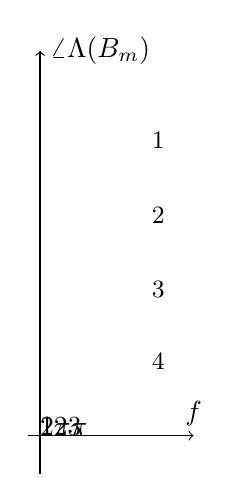
\begin{tikzpicture}[domain=0:3.1,samples=200]
      % \draw[very thin,color=gray] (-0.1,-1.1) grid (3.9,3.9);
      \begin{scope}[yscale=\scaleyphase,xscale=\scalex]
        \draw[->] (-0.25,0) -- (3.25,0) node[above] {$f$};
        \draw[->] (0,-0.7) -- (0,2*pi+0.7) node[right] {$\angle{\Lambda(B_m)}$};  
        \draw[thick] plot[] file {data/butterworth/data1.csv};
        \draw[thick] plot[] file {data/butterworth/data2.csv};
        \draw[thick] plot[] file {data/butterworth/data3.csv};
        \draw[thick] plot[] file {data/butterworth/data4.csv};
        % \node at (9.3,-1) {$0$};
        % \htick{2} node[pos=0.5,left] {$2$};
        \begin{scope}[font=\small]
          \node at (2.5,5.35) {$1$};
          \node at (2.5,4) {$2$};
          \node at (2.5,2.65) {$3$};
          \node at (2.5,1.35) {$4$};
        \end{scope}
      \end{scope}
      \begin{scope}[yscale=\scaleyphase]
        \htick{2*pi} node[pos=0.5,left] {$2\pi$};
        \htick{pi} node[pos=0.5,left] {$\pi$};
      \end{scope}
      \begin{scope}[xscale=\scalex]
        % \vtick{1/2} node[pos=0.5,below] {$\tfrac{1}{2}$};
        \vtick{1} node[pos=0.5,below] {$1$};
        \vtick{2} node[pos=0.5,below] {$2$};
        \vtick{3} node[pos=0.5,below] {$3$};
      \end{scope}
    \end{tikzpicture}
    \caption{Magnitude spectrum (top) and phase spectrum (bottom) of normalised Butterworth filters $B_1,B_2,B_3$ and $B_4$.} 
    \label{fig:butterworthspectrum}
  \end{figure}
}

The \term{cuttoff frequency} of the lowpass filter $B_m$ is defined as the positive real number $c$ such that $\abs{\Lambda B_m(f)}^2 < \tfrac{1}{2}$ for all $f > c$.  The normalised Butterworth filters have cuttoff frequency $c = 1\si{\hertz}$.  A lowpass Butterworth filter of order $m$ and cuttoff frequency $c$, denoted $B_m^c$, has transfer function
\[
\lambda B_m^c(s) = \lambda B_m\big(\tfrac{s}{c}\big) = \frac{1}{\prod_{i=1}^m(\tfrac{s}{2\pi c} - \beta_i)}.
\] 
The magnitude spectrum satisfies
\begin{equation}\label{eq:butterworthspectrum}
\sabs{\Lambda B_m^c(f)}^2 =  \sabs{\Lambda B_m\big(\tfrac{f}{c}\big)}^2 = \frac{1}{\big(\tfrac{f}{c}\big)^{2m} + 1} =  \frac{c^{2m}}{f^{2m} + c^{2m}}.
\end{equation}

A first order Butterworth filter $B_1^c$ has spectrum 
\[
\Lambda B_1^c(f) = \frac{1}{j\tfrac{f}{c} + 1} = \frac{c}{jf + c}.
\]  
Putting $\tfrac{1}{c} = 2\pi RC$ we find that this is the same as the spectrum of the RC electrical circuit (Figure~\ref{circ:seriesRC1}) or the active RC circuit after negation~\eqref{eq:specactiveRC}.  Thus, the RC electrical circuit is a first order Butterworth filter with cuttoff frequency $c = \tfrac{1}{2\pi RC}$.  In Test~\ref{test:activeRCspectrumtest} we constructed the active RC circuit with $R \approx 27\si{\kilo\ohm}$ and $C \approx 10\si{\nano\farad}$ and measured its magnitude spectrum.  The cuttoff frequency was $c = \tfrac{5\times10^4}{27\pi} \approx 589\si{\hertz}$.

A second order electrical Butterworth filter can be constructed using the Sallen-Key circuit described in Section~\ref{sec:active-circuits} and Figure~\ref{elec:sallenkey}.  The input voltage $x$ and output voltage $y$ of the Sallen-Key satisfy the differential equation~\eqref{eq:sallenkeydiffeq}
\[
x = y + C_2(R_1 + R_2) D y + R_1 R_2 C_1 C_2 D^2 y.
\]
The transfer function corresponding with this equation is
\[
\frac{1}{1 + C_2(R_1 + R_2) s + R_1 R_2 C_1 C_2 s^2}.
\]
The second order Butterworth filter $B_2^c$ has transfer function
\[
\Lambda B_2^c(s) = \frac{1}{(\tfrac{1}{2\pi c}s - \beta_1)(\tfrac{1}{2\pi c}s - \beta_2)},
\]
where $\beta_1 = \beta_2^* = e^{j3\pi/4}$.  Expanding the quadratic on the denominator gives
\[
\Lambda B_2^c(s) = \frac{1}{1 + \tfrac{1}{\sqrt{2} \pi c} s + \tfrac{1}{4\pi^2 c^2} s^2}.
\]
Choosing the resistors and capacitors of the Sallen-Key to satisfy 
\[
C_2(R_1 + R_2) = \frac{1}{ \sqrt{2} \pi c}, \qquad R_1 R_2 C_1 C_2 = \frac{1}{4\pi^2 c^2}
\]
leads to a second order Butterworth filter.  A convenient solution is to put $C_1 = 2C_2$ and $R_1 = R_2$.  This gives a second order Butterworth filter with cuttoff
\[
c = \frac{1}{\sqrt{2} \pi C_2(R_1+R_2)} =  \frac{1}{2\sqrt{2} \pi C_2 R_2}.
\]
In Test~\ref{test:butterworthfilter} we construct a second order Butterworth filter using a Sallen-Key and measure its spectrum.

Butterworth filters of orders larger than $m=2$ can be constructed by concatenating Sallen-Key circuits and RC circuits.  If $m$ is even then $m/2$ Sallen-Key circuits are required.  Each Sallen-Key is used to construct a conjugate pair of poles, that is, the $k$th Sallen-Key would have poles $2\pi c\beta_k$ and $2\pi c\beta_k^* = 2\pi c \beta_{m-k+1}$.  If $m$ is odd then $(m-1)/2$ Sallen-Key circuits and a single RC circuit (or active RC circuit) can be used.  The RC circuit is designed to have the real valued pole $\beta_{(m+1)/2} = 2\pi c$.

%\begin{randomfloat}
\begin{test}\label{test:butterworthfilter}
(\textbf{Butterworth filter})

We construct a second order Butterworth filter using the Sallen-Key circuit from Figure~\ref{elec:sallenkey} with capacitors $C_2 \approx 100\si{\nano\farad}$, $C_1 \approx 2C_2 \approx 200\si{\nano\farad}$ and resistors $R_1 \approx R_2 \approx 330\si{\ohm}$.  The cuttoff frequency is
\[
c = \frac{1}{2\sqrt{2} \pi C_2 R_2} \approx 3410\si{\hertz}.
\]
Sinusoids of the form
\[
\sin( 2 \pi f_k t ), \qquad f_k = \round{110 \times 2^{k/2}}, \;\; k = 1,2,\dots,13
\]
are input to the filter using a computer soundcard and the magnitude and phase spectrum are measured using the procedure described in Test~\ref{test:activeRCspectrumtest}.  Figure~\ref{fig:test:butterworthspectrum} shows the measurements (dots) plotted alongside the hypothesised magnitude spectrum
\[
\abs{\Lambda B_{2}^c(f)} = \sqrt{\frac{1}{(f/c)^4 + 1}}
\]
and the hypothesised phase spectrum $\angle{\Lambda B_{2}^c(f)}$.

% \begin{center}
% \captionsetup{type=figure}
% \includegraphics{tests/butterworth/plot-2.mps}
% 
% \end{center}

\end{test}
%\end{randomfloat}

\begin{figure}[p]
\centering
\begin{shaded}
  \begin{tikzpicture}
    \selectcolormodel{gray} 
    \begin{axis}[compat=newest,font=\small,height=8cm,width=12cm,ylabel={magnitude},xlabel={$f\;\;(\si{\hertz})$},legend style={draw=none,fill=none},xmax=10400,xmin=0]
      \addplot[mark=none,color=black,mark options={solid,fill=black,scale=0.7}] table[x index=0, y index=1] {tests/butterworth/hypothesised.csv};
      \addplot[mark=*,only marks,color=black,mark options={solid,fill=black,scale=0.7}] table[x index=0, y index=1] {tests/butterworth/measured.csv};
      \legend{$\abs{\Lambda(H)}$, measured}
    \end{axis}
  \end{tikzpicture}

  \begin{tikzpicture}
    \selectcolormodel{gray} 
    \begin{axis}[compat=newest,font=\small,height=8cm,width=12cm,ylabel={phase},xlabel={$f\;\;(\si{\hertz})$},legend style={draw=none,fill=none},xmax=10400,xmin=0]
      \addplot[mark=none,color=black,mark options={solid,fill=black,scale=0.7}] table[x index=0, y index=2] {tests/butterworth/hypothesised.csv};
      \addplot[mark=*,only marks,color=black,mark options={solid,fill=black,scale=0.7}] table[x index=0, y index=2] {tests/butterworth/measured.csv};
      \legend{$\angle\Lambda(H)$, measured}
    \end{axis}
  \end{tikzpicture}
\caption{Hypothesised magnitude spectrum $\abs{\Lambda(B_m^c)}$ (top) and phase spectrum $\angle{\Lambda(B_m^c)}$ (bottom) of the second order Butterworth filter and the measured magnitude and phase spectrum of the filter implemented with a Sallen-Key active electrical circuit (dots).}\label{fig:test:butterworthspectrum}
\end{shaded}
\end{figure}

\section{Complex valued sequences}

Let $x$ be a signal with Fourier transform $\hat{x} = \calF x$.  The signal $x$ is said to be \term{bandlimited} if there exists a positive real number $b$ such that 
\[
\hat{x}(f) = \calF x(f) = 0 \qquad \text{when $\abs{f} > b$}.
\]  
The value $b$ is called the \term{bandwidth} of the signal $x$.  For example, the $\sinc$ function is bandlimited with bandwidth $\tfrac{1}{2}$ because its Fourier transform $\calF \sinc(f) = \rect(f) = 0$ for all $\abs{f} > \tfrac{1}{2}$.
Bandlimited signals have a number of properties that make them suitable for representation and manipulation by a computer.  They are of particular importance for this reason.  Before we can study bandlimited signals we first require some properties of real and complex valued~\term{sequences}.

A \term{sequence} is a function with domain given by the integers $\ints$.  The value of a sequence $x$ at integer $n$ can be denoted by $x(n)$ but it is conventional to write $x_n$.  We are primarily interested in sequences that take complex (or real) values, that is, functions the set $\ints \to \complex$.  For example,
\[
\sin( \tfrac{\pi}{4} n), \qquad n^3, \qquad e^{-\sabs{n}/2}
\]
each denote a real (and so also complex) valued sequence.  In what follows the term~\term{sequence} will always mean a complex valued sequence unless otherwise stated.  Complex valued sequences are commonly called~\term{discrete time signals} and the $n$th element in the sequence is denoted by $x[n]$ using squared brackets~\citep{Oppenheiim_sigs_sys_1996}.  Here, we use the subscript notation $x_n$. This notation is also common~\citep{vetterli_fund_sig_proc,Rudin_real_and_complex_analysis}.
Sequences are plotted using vertical lines with dotted ends as in Figure~\ref{fig:realvaluedsequence} and have a number of properties analogous to the properties of signals (Section~\ref{sec:properties-signals}).

\begin{figure}[tp]
\centering
\def\minn{-4}
\def\maxn{4}
\def\scalex{0.6}
\def\step(#1){(#1>=0)} %step function
\def\deltaseq(#1){(#1==0)} %step function
\begin{tikzpicture}[domain=\minn:\maxn]
  \begin{scope}[xscale=\scalex]
    %\draw[very thin,color=gray] (-0.1,-1.1) grid (3.9,3.9);
    \draw[->] (\minn-0.5,0) -- (\maxn+0.5,0) node[above] {$n$};
    \draw[->] (0,-1.75) -- (0,1.75) node[left] {$\sin\big(\tfrac{\pi}{4} n\big)$};
    %\draw[color=black] plot[id=x] function{1/x^2} 
    %    node[right] {$f(t) = t^{-2}$};
    \draw[color=black,thick,ycomb,mark=*,mark options={xscale=1/\scalex,scale=0.75},samples=\maxn-\minn+1] plot function{sin(3.14159265359*x/4)};
    % \draw[color=black] plot[id=exp] function{0.05*exp(x)} 
    %    node[right] {$f(t) = \frac{1}{20} e^t$};
  \end{scope}
\end{tikzpicture} \;\;
\begin{tikzpicture}[domain=\minn:\maxn]
  \begin{scope}[xscale=\scalex]
    %\draw[very thin,color=gray] (-0.1,-1.1) grid (3.9,3.9);
    \draw[->] (\minn-0.5,0) -- (\maxn+0.5,0) node[above] {$n$};
    \draw[->] (0,-1.75) -- (0,1.75) node[left] {$e^{-\sabs{n}/2}$};
    \draw[color=black,ycomb,thick,mark=*,mark options={xscale=1/\scalex,scale=0.75},samples=\maxn-\minn+1] plot function{exp(-abs(x)/2)};
  \end{scope}
\end{tikzpicture}
\\ \vspace{0.5cm}
\begin{tikzpicture}[domain=\minn:\maxn]
  \begin{scope}[xscale=\scalex]
    %\draw[very thin,color=gray] (-0.1,-1.1) grid (3.9,3.9);
    \draw[->] (\minn-0.5,0) -- (\maxn+0.5,0) node[above] {$n$};
    \draw[->] (0,-0.75) -- (0,1.75) node[left] {$u_n$};
    %\draw[color=black] plot[id=x] function{1/x^2} 
    %    node[right] {$f(t) = t^{-2}$};
    \draw[color=black,thick,ycomb,mark=*,mark options={xscale=1/\scalex,scale=0.75},samples=\maxn-\minn+1] plot function{\step(x)};
    % \draw[color=black] plot[id=exp] function{0.05*exp(x)} 
    %    node[right] {$f(t) = \frac{1}{20} e^t$};
  \end{scope}
\end{tikzpicture} \;\;
\begin{tikzpicture}[domain=\minn:\maxn]
  \begin{scope}[xscale=\scalex]
    %\draw[very thin,color=gray] (-0.1,-1.1) grid (3.9,3.9);
    \draw[->] (\minn-0.5,0) -- (\maxn+0.5,0) node[above] {$n$};
    \draw[->] (0,-0.75) -- (0,1.75) node[left] {$\delta_n$};
    \draw[color=black,ycomb,thick,mark=*,mark options={xscale=1/\scalex,scale=0.75},samples=\maxn-\minn+1] plot function{\deltaseq(x)};
  \end{scope}
\end{tikzpicture}
\caption{Real valued sequences.  The bottom plots show that step sequence $u$ and the delta sequence $\delta$.} \label{fig:realvaluedsequence}
\end{figure}

A sequence $x$ is bounded if there exists a real number $M$ such that 
\[
\sabs{x_n} < M \qquad \text{for all $n \in \ints$}.
\]
Both $\sin( \tfrac{\pi}{4} n)$ and $e^{-\sabs{n}/2}$ are examples of bounded sequences, but $n^3$ is not bounded because its magnitude grows indefinitely as $n$ moves away from the origin.  A sequence $x$ is periodic if there exists a positive integer $T$ such that
\[
x_n = x_{n + kT} \qquad \text{for all integers $k$ and $n$.}
\] 
The smallest such $T$ is called the period.  The sequence $\sin( \tfrac{\pi}{4} n )$ is periodic with period $T=8$.  Neither $n^3$ or $e^{-n^2/4}$ are periodic.  
A sequence $x$ is even (or symmetric) if $x_n = x_{-n}$ for all $n \in \ints$ and odd (or antisymmetric) if $x_n = -x_{-n}$ for all $n \in \ints$.  Both $\sin(\frac{\pi}{4} n)$ and $n^3$ are odd and $e^{-\sabs{n}/2}$ is even.  
%%% BLERG, might also want conjugate symmetic?
%Every signal $x$ can be expressed as a sum $x = x_e + x_o$ where 
% \[
% x_e(t) = \tfrac{1}{2}\big( x(t) + x(-t) \big)
% \]
% is an even signal called the \term{even part} of $x$ and 
% \[
% x_o(t) = \tfrac{1}{2}\big( x(t) - x(-t) \big)
% \] 
% is an odd signal called the \term{odd part} of $x$.  For example, put $x(t) = e^{-t^2} + \sin(\pi t)$.  The even part of $x$ is $x_e(t) = e^{-t^2}$ and the odd part is $x_o(t) = \sin(\pi t)$.
%A complex valued sequence is \term{conjugate symmetric} if $x_n = x_-t)^* \qquad \text{for all $t \in \reals$,}
%\]
%where $*$ denotes the complex conjugate of a complex number.  Equivalently, $x$ is conjugate symetric if its real part is an even signal and its imaginary part is an odd signal.  Conversely, $x$ is \term{conjugate antisymmetric} if  
%\[
%x(t) = -x(-t)^* \qquad \text{for all $t \in \reals$,}
%\]  
%that is, if its real part is odd and its imaginary part is even.  For example, the signal $e^{-t^2} + j \sin(\pi t)$ where $j = \sqrt{-1}$ is conjugate symmetric and the signal $\tfrac{1}{2}t^{3} + j e^{-t^2}$ is conjugate antisymmetric.

A sequence $x$ is \term{right sided} if there exists a $T \in \reals$ such that $x_n = 0$ for all $t < T$.  Correspondingly $x$ is \term{left sided} if $x_n = 0$ for all $T > t$.  For example, the \term{step sequence} $u$ with $n$th element 
\begin{equation} \label{eq:stepsequence}
u_n = \begin{cases} 
1 & n \geq 0 \\
0 & n < 0 
\end{cases}
\end{equation}
is right sided  (Figure~\ref{fig:stepsided}).  The reflected sequence $u_{-n}$ is left sided.  A sequence is said to be of \term{finite support} or just \term{finite} if it is both left and right sided.  For example the sequence $\delta$ with $n$th element 
\begin{equation} \label{eq:deltasequence}
\delta_n = \begin{cases}
1 & n = 0 \\
0 & \text{otherwise},
\end{cases}
\end{equation}
called the \term{delta sequence}, is finite.  The delta sequence is analogous to the delta ``function'' introduced in Section~\ref{sec:conv-regul-syst}.  The delta ``function'' is not actually function, only a notational device.  Contrastingly, the delta sequence is a well defined sequence.

A sequence $x$ is \term{absolutely summable} if
\[
\|x\|_1 = \sum_{n \in \ints} \sabs{x_n} < \infty,
\]
that is, if the sum of absolute values of the elements in the sequence converges to a finite number.  The real number $\|x\|_1$ is commonly called the $\ell^1$-norm of $x$.  The sequences $\sin(\tfrac{\pi}{4} n)$ and $n^3$ are not absolutely summable, but $e^{-\abs{n}/2}$ is because
\[
\sum_{n \in \ints} \sabs{e^{-\sabs{n}/2}} = \sum_{n \in \ints} e^{-\sabs{n}/2} = 1 + \frac{2}{\sqrt{e} - 1}. \qquad \text{(Exercise~\ref{excer:sumgeomeabsn})}
\]
It is common to denote the set of absolutely summable sequences by $\ell^1$ or $\ell^1(\ints)$.  So, $e^{-\sabs{n}/2} \in \ell^1$ and $\sin(\tfrac{\pi}{4} n) \notin \ell^1$.

A sequence $x$ is \term{square summable} if
\[
\|x\|_2^2 = \sum_{n \in \ints} \sabs{x_n}^2 < \infty,
\]
that is, if the sum of squared magnitudes of the elements converges to a finite number.  The real number $\|x\|_2$ is commonly called the $\ell^2$-norm and its square $\|x\|^2_2$ the $\term{energy}$ of $x$.  The sequences $\sin(\tfrac{\pi}{4} n)$ and $n^3$ are not square summable, but $e^{-\abs{n}/2}$ is because 
\[
\sum_{n \in \ints} \sabs{e^{-\sabs{n}/2}}^2 = \sum_{n \in \ints} e^{-\abs{n}} = 1 + \frac{2}{e - 1}. \qquad \text{(Exercise~\ref{excer:sumgeomeabsn})}
\]
It is common to denote the set of square summable sequences by $\ell^2$.  So, $e^{-\sabs{n}/2} \in \ell^2$ and $\sin(\tfrac{\pi}{4} n) \notin \ell^2$.  If a sequence is absolutely summable then it is also square summable (Exercise~\ref{excer:sumsqreexp}).  The corresponding property is not true of signals, that is, absolutely integrable signals are not necessarily square integrable (Exercise~\ref{excer:absintnotsquareint}).


\section{Bandlimited signals}\label{sec:bandlimited-signals}

Let $b$ be a positive real number and let $x$ be a signal with Fourier transform $\hat{x} = \calF x$.  The signal $x$ is said to be \term{bandlimited} with \term{bandwidth} $b$ if 
\[
\hat{x}(f) = \calF x(f) = 0 \qquad \text{for all $\abs{f} > b$}.
\]  
For example, the sinc function $\sinc(t)$ that has Fourier transform $\rect(f)$ is bandlimited with bandwidth $b \geq \tfrac{1}{2}$.  Another example is the signal with Fourier transform given by a~\term{raised cosine}
\[
\hat{x}(f) = \rect(f) \big(1 + \cos( 2 \pi f )\big) = \begin{cases}
1 + \cos( 2\pi f ) & \abs{f} < \tfrac{1}{2} \\
0 & \text{otherwise}
\end{cases}
\]
that is bandlimited with bandwidth $b \geq \tfrac{1}{2}$.  The time domain signal is found by applying the inverse Fourier transform 
\[
x(t) = \sinc(t)+\tfrac{1}{2}\sinc(t+1)+\tfrac{1}{2}\sinc(t-1). \qquad \text{(Exercise~\ref{excer:raisedcosineft})}% = \frac{2b\sinc(bt)\cos(\pi b t)}{1 - 4 b^2 t^2}.
\]
Another example is the signal with Fourier transform given by the~\term{triangle pulse}
\[
\bigtriangleup(f) = \begin{cases}
f + 1 & -1 < f < 0 \\
1 - f & 0 \leq f < 1 \\
0 & \text{otherwise}
\end{cases}
\]
that is bandlimited with bandwidth $b \geq 1$.  The corresponding time domain signal is given by the square of the sinc function $\sinc^2(t)$ (Exercises~\ref{exer:triangle_pulse_ft}).  These bandlimited signals and their Fourier transforms are plotted in Figure~\ref{fig:bandlimittedsignals}.

It happens that bandlimited signals are never finite.  We can reasonably suppose that all signals ever encountered in practice are finite and so no signals encountered in practice are truely bandlimited.  However, many practically occuring signals are approximately bandlimited, that is, their Fourier transform is small for frequencies larger than some positive number $b$.  For example, in Test~\ref{test:ftlecturerec} the Fourier transform of an audio signal taken from a lecture recording is plotted  (Figure~\ref{fig:test:fouriertransformlecturevideo}).  This signal appears approximately bandlimited with bandwidth a little larger than \SI{8}{\kilo\hertz}.

% If $x$ is a bandlimited signal with bandwith $b$ then the time scaled signal $x(\alpha t)$ with $\alpha \neq 0$ has bandwidth $\abs{\alpha} b$ because, from the time scaling property of the Fourier transform,
% \[
% \calF(x(\alpha t), f) = \tfrac{1}{\alpha} \calF(x, \tfrac{f}{\alpha}) = 0 \qquad \abs{\frac{f}{\alpha}} < b.
% \]
% So, for example, the signal $\sinc(\alpha t)$ with $\alpha \neq 0$ has Fourier transform $\frac{1}{\alpha}\rect(\frac{f}{\alpha})$ and is bandlimited and bandwith $\tfrac{\alpha}{2}$.

% If $x$ is a bandlimited signal with bandwidth $b$ then the time shifted signal $T_\tau(x) = x(t - \tau)$ is also bandlimited with bandwidth $b$ because
% \[
% \calF(T_\tau(x), f) = \Lambda(T_\tau)\calF(x, f) = e^{-2\pi j \tau} \hat{x}(f) = 0
% \]
% when $\abs{f} > b$.  If $x$ and $y$ are bandmitted signals with bandwidth $b$ then the linear combination $ax + by$ for $a, b \in \complex$ is also bandlimited with bandwidth $b$ because
% \[
% \calF(ax + by, f) = a\calF(x, f) + a\calF(y, f) = a\hat{x}(f) + b\hat{y}(f) = 0
% \]
% when $\abs{f} > b$.  
% %If we let $S_b$ denote the set of bandlimited signals with bandwidth $b$ then we see that $S_b$ is a linear shift invariant space.
% It similary follows that if $x_1,\dots,x_N$ are bandlimited signals with bandwidth $b$ and $c_1,\dots,c_N$ are complex numbers then the signal $\sum_{n=1}^N c_n x_n$ is bandlimited with bandwidth $b$.  For example, the signal
% \[
% \sum_{n=1}^N c_n \sinc( 2 b t - n)
% \]
% has bandwidth $b$ because the signals $\sinc(2bt - n)$ have bandwidth $b$.  

A surprising result is that every square integrable bandlimited signal $x$ with bandwidth $b$ can be written as a sum of time-scaled and time-shifted $\sinc$ functions, that is, in the form
\begin{equation}\label{eq:sincinterformula}
 x(t) = \sum_{n \in \ints} c_n \sinc(F t - n)
 \end{equation}
%This sum is well defined since for fixed t the inside is the product of two square integrable sequences.
where $c$ is a square integrable complex valued sequence and $F = 2b$.  This is a consequence of a property of the space of square integrable signals $L_2$ called \term{completeness}~\cite[Theorem~3.11]{Rudin_real_and_complex_analysis}.  This property is sometimes also called the \term{Riesz-Fischer theorem}~\cite[page~91]{Rudin_real_and_complex_analysis}.  % If it happens that the sequence $c$ is also absolutely integrable then the order in which the terms in~\eqref{eq:sincinterformula} are summed does not matter and the convergence  
% \[
% x(t) = \sum_{n \in \ints} c_n \sinc(F t - n) \qquad a.e.
% \]
Evaluating the signal $x$ at integer multiples of $P = \tfrac{1}{F}$ we find that
\[
x(\ell P) = \sum_{n \in \ints} c_n \sinc( \ell - n ) = c_\ell
\]
because $\sinc( \ell - n)$ is equal to $1$ when $\ell = n$ and $0$ otherwise.  So, the elements of the sequence $c$ correspond with samples of the signal $x$ taken at integer multiples of $P = \tfrac{1}{F} = \tfrac{1}{2b}$, that is, $c_n = x(nP)$.  The positive real number $P$ is called the \term{sampling period} and its reciprical $F$ the \term{sampling rate}.  It follows that every square integrable bandlimited signal $x$ with bandwidth $b$ can be reconstructed from samples taken at rate $F = 2b$, that is,
\[
x(t) = \sum_{n \in \ints} x( n P ) \sinc(F t - n).
\]
This result known as the \term{Nyquist sampling theorem}.  %When a signal $x$ is not strictly bandlimited, but is approximately bandlimited, then this reconstruction method can produce an accurate approximation of $x$.
This theorem motivated use of this recontruction method in Tests~\ref{test:voltagedividertest1},~\ref{test:opampinvertingamplifiertest1},~\ref{test:activeRCtest}, and~\ref{test:activeRCtestagain}.

{
\def\sincf(#1){sin(pi*(#1))/(pi*(#1))} %step function
\begin{figure}[p]
  \centering
  \begin{tikzpicture}[domain=-4.8:4.8,samples=100]
    \begin{scope}[yscale=2,xscale=0.5]
      \draw[->] (-5.4,0) -- (5.4,0) node[above] {$t$};
      \draw[->] (0,-0.7) -- (0,1.3) node[above] {$\sinc(t)$};
      \draw[smooth,color=black,thick] plot function{\sincf(x)};
    \end{scope}
    \begin{scope}[yscale=2]
      \htick{1} node[pos=0.5,above left] {$1$};
    \end{scope}
    \begin{scope}[xscale=0.5]
      \vtick{1.0} node[pos=0.5,above right] {$1$};
      \vtick{-1.0} node[pos=0.5,above left] {$-1$};
    \end{scope}
  \end{tikzpicture} 
\;
\begin{tikzpicture}
  \begin{scope}[scale=2]
    \draw[->] (-1.35,0) -- (1.35,0) node[above] {$f$};
    \draw[->] (0,-0.7) -- (0,1.3) node[above] {$\rect(f)$};
    \draw[thick] (-1.2,0)--(-0.5,0)--(-0.5,1)--(0.5,1)--(0.5,0)--(1.2,0);
  \end{scope}
  \begin{scope}[yscale=2]
    \htick{1} node[pos=0.5,above left] {$1$};
  \end{scope}
  \begin{scope}[xscale=2]
    \vtick{0.5} node[pos=0.5,below] {$\tfrac{1}{2}$};
    \vtick{-0.5} node[pos=0.5,below] {$-\tfrac{1}{2}$};
  \end{scope}
\end{tikzpicture} 
\\
\vspace{1cm}
\begin{tikzpicture}
  \begin{scope}[yscale=2,xscale=0.5]
    % \def\sinc(#1){ifthenelse(abs(#1)>0.0001,sin(3.1415926*#1 r)/(3.1415926*#1),1)} %step function
    \draw[->] (-5.4,0) -- (5.4,0) node[above] {$t$};
    \draw[->] (0,-0.5) -- (0,1.3) node[above] {$\sinc^2(t)$};
    \draw[smooth,color=black,thick,domain=-4.8:4.8,samples=100] plot function{\sincf(x)*\sincf(x)};
  \end{scope}
\begin{scope}[yscale=2]
  \htick{1} node[pos=0.5,above right] {$1$};
\end{scope}
\begin{scope}[xscale=0.5]
  \vtick{1} node[pos=0.5,below] {$1$};
  \vtick{-1} node[pos=0.5,below] {$-1$};
\end{scope}
\end{tikzpicture}
\;
\begin{tikzpicture}
  \begin{scope}[yscale=2]
    % \def\sinc(#1){ifthenelse(abs(#1)>0.0001,sin(3.1415926*#1 r)/(3.1415926*#1),1)} %step function
    \draw[->] (-2.7,0) -- (2.7,0) node[above] {$f$};
    \draw[->] (0,-0.5) -- (0,1.3) node[above] {$\bigtriangleup(f)$};
    \draw[color=black,thick,domain=-1:0,samples=2] plot function{x+1};
    \draw[color=black,thick,domain=0:1,samples=2] plot function{1-x};
    \draw[thick] (-2.4,0)--(-1,0);
    \draw[thick] (1,0)--(2.4,0);
    \htick{1} node[pos=0.5,above right] {$1$};
  \end{scope}
  \vtick{1} node[pos=0.5,below] {$1$};
  \vtick{-1} node[pos=0.5,below] {$-1$};
\end{tikzpicture}
\\
\vspace{1cm}
\begin{tikzpicture}
\begin{scope}[yscale=2,xscale=0.5]
    \draw[->] (-5.4,0) -- (5.4,0) node[above] {$t$};
    \draw[->] (0,-0.35) -- (0,1.2) node[above,font=\footnotesize] {$\sinc(t) + \tfrac{1}{2}\sinc(t+1) + \tfrac{1}{2}\sinc(t-1)$};    
    \draw[smooth,color=black,thick,domain=-4.8:4.8,samples=100,line cap=round] plot function{\sincf(x)+0.5*\sincf(x-1)+0.5*\sincf(x+1)};
  \end{scope}
  \begin{scope}[xscale=0.5]
    \vtick{-2.0} node[pos=0.5,below] {$-2$};
    \vtick{2} node[pos=0.5,below] {$2$};
\end{scope}
  \begin{scope}[yscale=2]
    \htick{1} node[pos=0.5,above left] {$1$};
  \end{scope}
\end{tikzpicture}
\; 
\begin{tikzpicture}
  \begin{scope}[xscale=2]
    \draw[->] (-1.35,0) -- (1.35,0) node[above] {$f$};
    \draw[->] (0,-0.7) -- (0,2.4) node[above] {$\rect(f) + \rect(f)\cos( 2\pi f )$};
    \draw[thick] (-1.2,0)--(-0.5,0);  
    \draw[thick] (0.5,0)--(1.2,0);
    \draw[smooth,color=black,thick,domain=-0.5:0.5,samples=50] plot function{1 + cos(2*3.1415926*x)};
\vtick{0.5} node[pos=0.5,below] {$\tfrac{1}{2}$};
    \vtick{-0.5} node[pos=0.5,below] {-$\tfrac{1}{2}$}; 
\end{scope}
    \htick{2} node[pos=0.5,above left] {$2$};
\end{tikzpicture} 
\caption{Bandlimited signals $\sinc(t)$, $\sinc^2(t)$, and $\sinc(t) + \tfrac{1}{2}\sinc(t+1) + \tfrac{1}{2}\sinc(t-1)$ with bandwidth $\tfrac{1}{2}$, $1$, and $\tfrac{1}{2}$ respectively.} \label{fig:bandlimittedsignals}
\end{figure}
}

\section{The discrete time Fourier transform}

Let $x$ be a square integrable bandlimited signal with bandwidth $b$ and let $c$ be the square summable sequence containing samples of $x$ at sampling rate $F = \tfrac{1}{P} = 2b$, that is, $c_n = x(nP)$.  Suppose temporarily that $c$ is also absolutely summable.  
From~\eqref{eq:sincinterformula}, the Fourier transform of $x$ is %BLERG this is using completeness of L_2
\begin{align}
\hat{x}(f) = \calF x(f) &= \sum_{n \in \ints} c_n \calF(\sinc(F t - n))(f)  \label{eq:ftanddftrelationshipswapsumf} \\
&= P \rect( f P ) \sum_{n \in \ints} c_n e^{-j 2\pi P n f } \nonumber \\
&= P \rect( f P ) \calD c(Pf) \qquad \label{eq:ftanddftrelationship}
\end{align}
where
\begin{equation}\label{eq:disctransintro}
\calD c(f) = \sum_{n \in \ints} c_n e^{-j 2\pi n f}
\end{equation}
is called the~\term{discrete time Fourier transform} of the sequence $c$.  The interchange of Fourier transformation and summation on line~\eqref{eq:ftanddftrelationshipswapsumf} can be justified using \term{Lebesgue's dominated convergence theorem}~\cite[Section~1.34]{Rudin_real_and_complex_analysis} (Exercise~\ref{exer:ftdftswapsummationldct}).  
We write $\hat{c} = \calD c$ for the discrete time Fourier transform of $c$.  Under our assumption that $c$ is absolutely summable
\[
\abs{\calD c(f)} \leq \sum_{n \in \ints} \abs{c_n e^{-j 2\pi n f}} = \sum_{n \in \ints} \abs{c_n} = \|c\|_1 < \infty
\]
and so the discrete Fourier transform $\calD c(f)$ is finite for all $f$.  A discrete time Fourier transform can also be assigned to sequences that are only square integrable and not necessarily absolutely integrable.  In this case one interprets the sum in~\eqref{eq:disctransintro} as
\[
\calD c(f) = \lim_{N \to \infty} \sum_{n = -N}^N c_n e^{-j 2\pi n f}.
\]
This is analogous to how the Fourier transform of a square integrable signal was assigned using the Cauchy principal value~\eqref{eq:cauchyprinvalint}.  The relationship~\eqref{eq:ftanddftrelationship} still holds in this case provided that equality is weakened to equality almost everywhere.% that is, if $c$ is square integrable, then $\hat{x}(t) = P \rect( f P ) \calD c(Pf)$
%TODO Introduce completeness in an advanced section?

The discrete time Fourier transform $\hat{c} = \calD c$ is a periodic function from $\reals \to \complex$, that is, $\hat{c}$ is a periodic signal.  The fundamental period of $\hat{c}$ is $1$.  The above equations relate the Fourier transform of the bandlimited signal $x$ to the discrete time Fourier transform of its sequence of samples $c$.  In Test~\ref{test:ftlecturerec} we compute the Fourier transform of a \SI{20}{\second} segment of audio from a lecture recording.  In Test~\ref{test:butterworthfilteredlecturerec} we pass the audio signal through the Butterworth filter constructed in Test~\ref{test:butterworthfilter} and plot the Fourier transform of the response.

The sequence of samples $c_n = x(nP)$ can be recovered by evaluating the inverse Fourier transform
\begin{align*}
c_n = x(nP) &= \calF^{-1}\hat{x}(nP) \\
&= \int_{-\infty}^\infty P \rect(Pf) \calD c(Pf) e^{j2\pi f nP} df \\
&= P \int_{-F/2}^{F/2} \hat{c}(Pf) e^{j2\pi f nP } df \\
&= \int_{-1/2}^{1/2} \hat{c}(\gamma) e^{j 2\pi \gamma n } d\gamma \qquad \text{(change variable $\gamma = fP$)}.
\end{align*}
We obtain the following relationship between the square integrable sequence $c$ and its periodic discrete time Fourier transform $\hat{c} = \calD c$,
\[
c_n = \int_{-1/2}^{1/2} \hat{c}(f) e^{j 2\pi f n } df.
\]
The right hand side of this expression is called the~\term{inverse discrete time Fourier transform}.  %The inverse discrete Fourier transform is a sequence, that is, a function from $\ints$ to $\complex$.  
The element $c_{-n}$ is also called the $n$th~\term{Fourier coefficient} of the periodic function $\hat{c}$.

\begin{test}\label{test:ftlecturerec}
(\textbf{The Fourier transform of a lecture recording})

In this test we consider a \SI{20}{\second} segment of audio taken from the lecture video \href{www.itr.unisa.edu.au/~mckillrg/videos/lectures/signalsandsystems2014/ch1sec3.mp4}{\texttt{ch1sec3.mp4}}.  
%available at:
% %\vspace{0.1cm}
% \begin{center}
% \parbox[][][c]{12cm}{
% \url{www.itr.unisa.edu.au/~mckillrg/videos/lectures/signalsandsystems2014/ch1sec3.mp4}
% }
% \end{center}
% %\vspace{0.1cm}
This \SI{34.8}{\mega\byte} file contains both compressed video (H.264 codec) and audio (mp3 codec) of duration \SI{23}{\minute} and \SI{36}{\second}.  The audio is mono and sampled at rate $F = \SI{22050}{\hertz}$.  The \href{https://www.ffmpeg.org/}{\texttt{ffmpeg}} program is used to extract a \SI{20}{\second} segment of audio starting at time \SI{85}{\second} and ending at time \SI{105}{\second}.  The segment is decompressed to wav format.  The command used is:
%\vspace{0.1cm}
\begin{center}
\parbox[][][c]{10cm}{
\texttt{ffmpeg -i ch1sec3.mp4 -ss 85 -t 20 audio.wav}
}
\end{center}
%\vspace{0.1cm}
The resulting file \texttt{audio.wav} is \SI{882}{\kilo\byte} in size and contains $N = 440998$ samples that we denote by $c_0,c_1,\dots,c_{N-1}$.  Each sample takes a value in the interval $[-1,1]$.  We put $c_n = 0$ when $n < 0$ or $n \geq N$.  The reconstructed audio signal is given by
\[
x(t) = \sum_{n \in \ints} c_n \sinc(Ft - n) = \sum_{n=0}^{N-1} c_n \sinc(Ft - n).
\]
From~\eqref{eq:ftanddftrelationship} the Fourier transform of this signal is $\hat{x}(f) = P \rect(P f) \hat{c}(Pf)$ where 
\begin{equation}\label{eq:dftsumNterms}
\hat{c}(f) = \calD c(f) = \sum_{n \in \ints} c_n e^{-j 2\pi n f}  = \sum_{n = 0}^{N-1} c_n e^{-j 2\pi n f}
\end{equation}
is the discrete time Fourier transform of the sequence of samples.  Figure~\ref{fig:test:fouriertransformlecturevideo} shows a plot of the magnitude of the Fourier transform for frequencies in the interval \SI{-12}{\kilo\hertz} to \SI{12}{\kilo\hertz}.  The plot is constructed by evaluting $\abs{\hat{c}(f)}$ at all $K = 1201$ frequencies
\[
f_k = -12000 + 20k \qquad k = 0, \dots, K-1,
\]
that is, from \SI{-12}{\kilo\hertz} to \SI{12}{\kilo\hertz} in steps of \SI{20}{\hertz}.  It takes approximately \SI{137}{\second} to compute the Fourier transform at all of these frequencies.  Evaluating the Fourier transform at a particular frequency requires calculating and accumlating each of the $N$ terms in the sum~\eqref{eq:dftsumNterms}.  We hypothesise it to take approximately
\[
\frac{\SI{137}{\second}}{NK} \approx \SI{260}{\nano\second}
\]
to compute each term.   The computer used is an Intel Core 2 running at \SI{2.4}{\giga\hertz} and the software is written in the \href{http://scala-lang.org/}{\texttt{Scala}} programming language.

The audio recording contains human voice that primarily resides at lower frequencies below \SI{5}{\kilo\hertz}.  Audible in the recording is a faint high pitched hum.  The cause of this is unknown.  It might be a feature of the (probably low quality) webcam microphone used to record the audio.  This hum is represented in Figure~\ref{fig:test:fouriertransformlecturevideo} by the spikes occurring at approximately $\pm\SI{8}{\kilo\hertz}$ and also by the region between \SI{4900}{\hertz} and \SI{5900}{\hertz} where the magnitude of the Fourier transform is elevated.  Figure~\ref{fig:test:fouriertransformlecturevideozoomed} is a plot of the Fourier transform for frequencies from \SI{7998}{\hertz} to \SI{8002}{\hertz} in steps of \SI{5}{\milli\hertz}.  This gives a high resolution view of the spike that occurs near \SI{8}{\kilo\hertz}.  The magnitude of the Fourier transform is precisely zero for frequencies $\abs{f} > F/2 = \SI{11025}{\hertz}$ due to $\rect(Pf)$ occurring in the definition of $\hat{x}$.  However, in Figure~\ref{fig:test:fouriertransformlecturevideo} it is apparent that the Fourier transform is small if $\abs{f}$ is a little larger than $\SI{8}{\kilo\hertz}$.  This audio signal appears approximately bandlimited with bandwidth a little larger $\SI{8}{\kilo\hertz}$.

% \begin{center}
% \captionsetup{type=figure}
% %\includegraphics{tests/fouriertransformlecturevideo/plot-1.mps}
%   \begin{tikzpicture}
%     \selectcolormodel{gray} 
%     \begin{axis}[compat=newest,font=\small,height=8cm,width=12cm,ylabel={$\abs{\hat{x}(f)}$},xlabel={$f\;\;(\si{\hertz})$},legend style={draw=none},xmin=4900,xmax=5900]
%       \addplot+[mark=none,color=black,mark options={solid,fill=black,scale=0.7}] table[x index=0, y index=1] {tests/fouriertransformlecturevideo/ft4900.csv};
%     \end{axis}
%   \end{tikzpicture} 
% \captionof{figure}{A plot of the magnitude of the Fourier transform zoomed in on the the interval $[\SI{4900}{\hertz}, \SI{5900}{\hertz}]$.}\label{fig:test:fouriertransformlecturevideozoomed}
% \end{center}

\end{test}

\begin{randomfloat}[p]
\begin{shaded}
\begin{center}
%\includegraphics{tests/fouriertransformlecturevideo/plot-1.mps}
  \begin{tikzpicture}
    \selectcolormodel{gray} 
    \begin{axis}[compat=newest,font=\small,height=8cm,width=12cm,ylabel={$\abs{\hat{x}(f)}$},xlabel={$f\;\;(\si{\hertz})$},legend style={draw=none},xmin=-11800,xmax=11800]
      \addplot+[mark=none,color=black,mark options={solid,fill=black,scale=0.7}] table[x index=0, y index=1] {tests/fouriertransformlecturevideo/ft.csv};
    \end{axis}
  \end{tikzpicture}
\captionsetup{type=figure}
\captionof{figure}{Magnitude of the Fourier transform of \SI{20}{\second} of audio from a lecture recording.  The human voice signal is primarily contained in the low frequency region below \SI{5}{\kilo\hertz}.  The spikes occurring at approximately $\pm\SI{8}{\kilo\hertz}$ and the region between \SI{4900}{\hertz} and \SI{5900}{\hertz} where the magnitude is elevated are audible in the recording as a high pitched hum.}\label{fig:test:fouriertransformlecturevideo}
\end{center}

\begin{center}
%\includegraphics{tests/fouriertransformlecturevideo/plot-1.mps} 
  \begin{tikzpicture}
    \selectcolormodel{gray} 
    \begin{axis}[compat=newest,font=\small,height=8cm,width=12cm,ylabel={$\abs{\hat{x}(f)}$},xlabel={$f\;\;(\si{\hertz})$},legend style={draw=none},xmin=7997.9,xmax=8002.1,xtick={7998,7999,8000,8001,8002},x tick label style={/pgf/number format/.cd,set thousands separator={},fixed}]
      \addplot+[mark=none,color=black,mark options={solid,fill=black,scale=0.7}] table[x index=0, y index=1] {tests/fouriertransformlecturevideo/ft8k.csv};
    \end{axis}
  \end{tikzpicture}
\captionsetup{type=figure} 
\captionof{figure}{A plot of the magnitude of the Fourier transform zoomed in on the spike at \SI{8}{\kilo\hertz}.}\label{fig:test:fouriertransformlecturevideozoomed}
\refstepcounter{figure} %for some reason the figure counter does not step here. Might have something to do with randomfloat.  Steping manually
\end{center}
\end{shaded}
\end{randomfloat}

\begin{randomfloat}[p]
\begin{test}\label{test:butterworthfilteredlecturerec}
(\textbf{Butterworth filtered lecture recording})

We consider again the \SI{20}{\second} audio signal from Test~\ref{test:ftlecturerec}.  In this test we pass this signal through the second order Butterworth filter from Test~\ref{test:butterworthfilter} with cuttoff frequency approximately \SI{3041}{\hertz}.  The output of the Butterworth filter is fed back to the soundcard input and recorded at \SI{22050}{\hertz}.  The recorded samples are written to the file \texttt{filtered.wav}.  Listening to \texttt{filtered.wav} confirms that the high pitched hum is weaker than it is in the original audio signal.  The Fourier transform of the Butterworth filtered signal is plotted in Figure~\ref{fig:test:butterworthedfouriertransformlecturevideo}.  This figure is constructed by the same procedure as used for Figure~\ref{fig:test:fouriertransformlecturevideo} from Test~\ref{test:ftlecturerec}.  Observe that the spikes occurring at approximately $\pm\SI{8}{\kilo\hertz}$ are less prominent than in Figure~\ref{fig:test:fouriertransformlecturevideo}.

\begin{center}
%\includegraphics{tests/fouriertransformlecturevideo/plot-1.mps}
  \begin{tikzpicture}
    \selectcolormodel{gray} 
    \begin{axis}[compat=newest,font=\small,height=8cm,width=12cm,ylabel={$\abs{\hat{x}(f)}$},xlabel={$f\;\;(\si{\hertz})$},legend style={draw=none},xmin=-11800,xmax=11800]
      \addplot+[mark=none,color=black,mark options={solid,fill=black,scale=0.7}] table[x index=0, y index=1] {tests/butterworthfilteredlecturerecording/ft.csv};
    \end{axis}
  \end{tikzpicture}
\captionof{figure}{Magnitude of the Fourier transform of \SI{20}{\second} of audio from Test~\ref{test:ftlecturerec} after being passed through the second order Butterworth filter from Test~\ref{test:butterworthfilter} with cuttoff frequency approximately \SI{3041}{\hertz}.  The magnitude of the Fourier transform at higher frequencies is attenuated when compared with the Fourier transform of the original audio signal (Figure~\ref{fig:test:fouriertransformlecturevideo}).  In particular, the spikes occurring at approximately $\pm\SI{8}{\kilo\hertz}$ are less prominent than in Figure~\ref{fig:test:fouriertransformlecturevideo}.  The high pitched hum that is audible in the original audio signal is significantly weaker in the Butterworth filtered audio signal.}\label{fig:test:butterworthedfouriertransformlecturevideo}
\end{center}

\end{test}
\end{randomfloat}

\clearpage

\section{The fast Fourier transform}\label{sec:fast-four-transf}

In Test~\ref{test:ftlecturerec} the Fourier transform of a \SI{20}{\second} audio signal consisting of $N=440998$ consecutive samples was evaluated.  This scenario where only a finite number, say $N$, of consecutive samples of a signal is available is common in practice.  Let $c$ be a sequence with elements $c_0,c_1,\dots, c_{N-1}$ equal to the $N$ samples.  A convenient assumption is that the remaining samples are equal to zero, that is, $c_n = 0$ when $n < 0$ or $n \geq N$.  This assumption was made in Test~\ref{test:ftlecturerec}.

With this assumption the discrete time Fourier transform of the sequence $c$ is given by the finite sum
\[
\hat{c}(f) = \calD c(f) = \sum_{n \in \ints} c_n e^{-j 2\pi n f}  = \sum_{n = 0}^{N-1} c_n e^{-j 2\pi n f}.
\]
The values of $\hat{c}(f)$ for $f$ a multiple of $\tfrac{1}{N}$ have a number of convenient properties.  Denote these values by
\begin{equation}\label{eq:dftdefn}
(\calD_N c)_k = \calD c\big(\tfrac{k}{N}\big) = \sum_{n = 0}^{N-1} c_n e^{-j 2\pi n k/N} \qquad k \in \ints. 
\end{equation}
This is called the~\term{discrete Fourier transform} (as opposed to the discrete \emph{time} Fourier transform).  The discrete Fourier transform $\calD_N c$ is a sequence with elements given by the discrete time Fourier transform $\calD c$ evaluated at multiples of $\tfrac{1}{N}$.  As usual we include write $\calD_N c_k$ to denote the value of $\calD_N c$ at $k \in \ints$.  We will regularly include brackets and use $(\calD_N c)_k$ to denote this value.  The positive integer $N$ is called the~\term{length} of the transform.  In practical applications $N$ often corresponds with the number of samples of a signal that have been obtained.

%\renewcommand{\mod}{\operatorname{mod}}

The discrete Fourier transform is a periodic sequence with period $N$ as a result of the discrete time Fourier transform $\hat{c} = \calD c$ having period $1$, that is,
\[
(\calD_N c)_k = \hat{c}\left( \frac{k}{N} \right) = \hat{c}\left( \frac{k + mN}{N} \right) = (\calD_N c)_{k+mN} \;\;\; \text{for all $k,m\in\ints$}.
\]
% It follows that
% \[
%  \hat{d}_{k} = \hat{d}_{k \bmod N} \qquad k \in \ints
%  \]
% where $k \bmod N$ denotes $k$ taken modulo $N$ into the set $\{0,1\dots,N-1\}$.
Because of this it is sufficient to know only $(\calD_N c)k$ for $k = 0,\dots,N-1$ in order to know the entire sequence $\calD_N c$.  Given $d = \calD_N c$ the original samples $c_0, \dots, c_{N-1}$ can be recovered by 
\[
%\begin{equation}\label{eq:inversedft}
c_n = (\calD_N^{-1}d)_n = \frac{1}{N}\sum_{k = 0}^{N-1} d_k e^{j 2\pi n k / N} \qquad n = 0, \dots, N-1.
%\end{equation}
\]
This is called the \term{inverse discrete Fourier transform} (Excersise~\ref{exer:inversedft}). Taking complex conjugates on both sides gives
\[
c_n^* = \frac{1}{N} \sum_{k = 0}^{N-1} d_k^* e^{-j 2\pi n k / N} = \frac{1}{N} \calD_N(d^*, n)  \qquad n = 0, \dots, N-1.
\]
A practical consequence of this is that the inverse discrete Fourier transform can be evaluted by applying the complex conjugate, taking the discrete Fourier transform, applying the complex conjugate again, and finally dividing by $N$.  That is, if $d$ is a sequence, then $\calD_N^{-1} d = \tfrac{1}{N}\calD_N^* d^*$.

Suppose that we wish to evaluate the discrete Fourier transform $\calD_N c$ of the \SI{20}{\second} audio signal comprising of $N=440998$ samples from Test~\ref{test:ftlecturerec}.  In Test~\ref{test:ftlecturerec} we hypothesised that approximately $\SI{260}{\nano\second}$ are required to compute each term in the sum~\eqref{eq:dftsumNterms}.  We require to compute the sum for each $k = 0,\dots,N-1$ and so we might expect that
\begin{equation}\label{eq:runtimefftformulaapprox}
N^2 \times \SI{260}{\nano\second} \approx \SI{50565}{\second} \approx 14 \; \text{hours}
\end{equation}
will be required to compute $\calD_N c$ for this \SI{20}{\second} audio signal!  A primary cause of this lengthy computation time is the quadratic term $N^2$ that occurs in the expression above.  The amount of time required grows proportionally with the square of the length of the transform.  Suppose that instead of \SI{20}{\second} of audio we have $1$ hour and $N = 60 \times 60 \times 22050 = 79380000$ samples.  The amount of time required in this case is approximated by $N^2 \times \SI{260}{\nano\second}  \approx 52$ years!

Computing the discrete Fourier transform by direct application of the formula~\eqref{eq:dftdefn} is too slow when $N$ is large.  Fortunately, much faster algorithms exist.  The algorithms are appropriately called \term{fast Fourier transforms}.  The specific algorithm used depends on $N$.  The simplest case is when $N = 2^m$ is a power of $2$.  In this case an algorithm attributed to~\citet{Cooley_tukey_1965} can be used.  %The algorithm is called the \term{radix-2 decimation in time} fast Fourier transform.  
When $N = 2^m$ is divisible by $2$ the sum in~\eqref{eq:dftdefn} can be split into two parts corresponding with $n$ being even or odd,
\begin{equation}\label{eq:DNsplitevenodd}
(\calD_N c)_k =  \sum_{n = 0}^{N/2-1} c_{2n} e^{-j 2\pi (2n)k/N} +  \sum_{n = 0}^{N/2-1} c_{2n+1} e^{-j 2\pi (2n+1) k/N}.
\end{equation}
Put $M = N/2$ and let $p$ be the sequence with elements $p_n = c_{2n}$, that is, the elements of $p$ are the even indexed elements of $c$.  Now the first term in~\eqref{eq:DNsplitevenodd} can be written in the form
\[
\sum_{n = 0}^{N/2-1} c_{2n} e^{-j 2\pi (2n)k/N}  = \sum_{n = 0}^{M-1} p_n e^{-j 2\pi n k/M} = (\calD_M p)_k,
\]
that is, this term is the discrete Fourier transform of length $M = N/2$ of the sequence $p$.  Let $q$ be the sequence with elements $q_n = c_{2n+1}$, that is, $q$ contains the odd indexed elements of $c$.  The second term in~\eqref{eq:DNsplitevenodd} can be written in the form
\begin{align*}
\sum_{n = 0}^{N/2-1} c_{2n+1} e^{-j 2\pi (2n+1) k/N} &= e^{-j 2\pi k / N} \sum_{n = 0}^{M-1} q_n e^{-j 2\pi n k/M} \\
&= e^{-j 2\pi k / N} (\calD_{M}q)_k,
\end{align*}
that is, this term is the discrete Fourier transform of length $M=N/2$ of the sequence $q$ multiplied by $e^{-j 2\pi k / N}$.  Combining these results we have
\[
(\calD_N c)_k = (\calD_{N/2}p)_k + e^{-j 2\pi k / N} (\calD_{N/2} q)_k.
\]
We see that the discrete Fourier transform $\calD_N c$ can be evaluated by computing two smaller discrete Fourier transforms $\calD_{N/2} p$ and $\calD_{N/2} q$ of length $N/2$.  Both of these smaller transforms are sequences that are periodic with period $N/2$ and so it is sufficient to know their values only for $k = 0,\dots,\tfrac{N}{2}-1$.  % Thus,
% \[
% \calD_N(c, k) = \calD_{N/2}(e, k \bmod \tfrac{N}{2}) + e^{-j 2\pi k / N} \calD_{N/2}(o, k \bmod \tfrac{N}{2}) \qquad k \in \ints. 
% \]
These $N/2$ length transforms can in turn be computed by two transforms of length $N/4$ and so on until transforms of length $1$ are obtained.  In this case $(\calD_{1} c)_k = \sum_{n = 0}^{0} c_n e^{-j 2\pi n k } = c_0$  for all $k \in \ints$.  

The computational cost of this procedure can be analysed as follows.  Suppose that $C_N$ is the number of complex arithmetic operations (complex additions and multiplications) required to compute the discrete Fourier transform $\calD_N c$ of length $N = 2^m$.  The computation requires calculation of two transforms of length $N/2$ followed by $N$ complex multiplications and $N$ additions.  The multiplications arise from the multiplication of $(\calD_{N/2}q)_k$ by $e^{-j 2\pi k / N}$ and the additions arise from summing the result of this product with $(\calD_{N/2}p)_k$.  The number of operations satisfies
\[
C_N = 2C_{N/2} + 2N \qquad N \geq 2.
\]
Because $(\calD_1 c)_k = c_0$ we have $C_1 = 0$, that is, computing a discrete Fourier transform of length $1$ requires no complex operations at all.  Putting $a_m = C_{2^m}$ we have
\begin{equation}\label{eq:recursiveeqcomplexityfft}
a_0 = C_1 = 0 \qquad a_m = 2 a_{m-1} + 2^{m+1} \;\;\; m \geq 1.
\end{equation}
This type of recursive equation is called a~\term{difference equation} and will be studied further in Section~\ref{sec:difference-equations}.  %We will learn how to solve such equations in Section~\ref{sec:difference-equations}.  For now we simply state the solution.  
Exercise~\ref{exer:fftcomplexity} shows that
\[
C_{N} = a_{m} = 2^{m+1}m = 2N\log_2 N.
\]

Observe that the number of operations (and hence the amount of time required) grows proportionally to $N\log_2 N$ rather than $N^2$.  Suppose that each complex operation requires no more than \SI{260}{\nano\second}.  For the \SI{20}{\second} audio signal consisting of $N = 440998$ samples the amount of time required will be less than
\begin{equation}\label{eq:runtimefftcooleytukeyapprox}
2N \log_2 N \times \SI{260}{\nano\second} \approx \SI{4.3}{\second}.
\end{equation} 
This is more reasonable than 14 hours!  If instead we have 1 hour of audio and $N = 79380000$ samples the amount of time required is hypothesised to be less than $\SI{1084}{\second} \approx \SI{18}{\minute}$.  This is very reasonable when compared with the $52$ years hypothesised to be required by direct application of formula~\eqref{eq:dftdefn}.  In practice the computation time will vary based on the computer used and the specific algorithm implementation.  Nevertheless, these numbers indicate that a fast Fourier transform of large length can be computed within a reasonable amount of time.  This is not possible by direct application of formula~\eqref{eq:dftdefn}.  Test~\ref{test:fastftbenchmarks} compares the practical running time of various discrete Fourier transform implementations.

In the above computation of run times we have neglected that the fast Fourier transform we have described required the length $N$ to be a power of two.  Other algorithms exist for the case when $N$ is not a power of two~\citep{Rader_fft_prime_1968,Bluestein_fft_prime_1968,FrigoJohnson_fftw_2005}.  These algorithms deliver similarly dramatic computational savings.  Even so, the restriction of the length to a power of $2$ is often not a significant drawback in practical applications.  Consider again the example from Test~\ref{test:ftlecturerec} with $N=440998$ samples.  Denote by 
\[
L = 2^{\ceil{\log_2 N}} = 2^{19} = 524288
\] 
the smallest power of $2$ greater than $N$.  We can use the fast Fourier transform algorithm described to compute the discrete Fourier transform $D_L c$ of length $L$.  This transform is a sequence with period $L$ and elements 
\[
(\calD_L c)_k = \hat{c}\left(\frac{k}{L}\right) = \sum_{n = 0}^{L-1} c_n e^{-j 2\pi n k/L} = \sum_{n = 0}^{N-1} c_n e^{-j 2\pi n k/L} \qquad k \in \ints.
\]
The second sum follows from our assumption that $c_n = 0$ for $n \geq N$.  The elements of $\calD_L c$ are the values of the discrete time Fourier transform $\hat{c}$ at multiples of $\tfrac{1}{L}$ rather than $\tfrac{1}{N}$.  This fact is often of no significant consequence and can even be of benefit for some applications~\citep{Quinn2001,Quinn2008maximizing_the_periodogram}.  The original samples $c_0, \dots, c_{N-1}$ can still be recovered by application of the inverse transform of length $L$, that is, 
\[
c_n = (\calD_L^{-1} \calD_L c)_n \qquad  n = 0, \dots, N-1.
\]  
This procedure of increasing the length of the transform is often called \term{zero padding} on account of the fact that the samples $c_N, c_{N+1}, \dots, c_{L-1}$ are assumed to be zero.  Test~\ref{test:fftlecturerec} presents a practical example of zero padding for the purpose of filtering the \SI{20}{\second} audio recording from Test~\ref{test:ftlecturerec}.

%In Test~\ref{test:ftlecturerec} the Fourier transform of a \SI{20}{\second} audio signal consisting of $N=440998$ samples was evaluated at $K=1201$ different frequencies.  It was concluded that approximately \SI{260}{\nano\second} was required to computed each term in the sum defining the Fourier transform~\eqref{eq:dftsumNterms}.  Suppose now that we wish to compute the Fourier transform of \SI{23}{\minute} and \SI{36}{\second} audio recording consisting of $N=?$ sampl

\begin{test}\label{test:fastftbenchmarks}
(\textbf{Benchmarking the fast Fourier transform})

In this test we compare the computational complexity of practical implementations of the discrete Fourier transform.  Three differenent implementations are compared: a direct implementation by formula~\eqref{eq:dftdefn}, an implementation of  the fast Fourier transform of~\citet{Cooley_tukey_1965} when the length $N = 2^m$ is a power of 2 as described in Section~\ref{sec:fast-four-transf}, and an implementation from an optimised fast Fourier transform library called \href{https://github.com/wendykierp/JTransforms}{\texttt{JTransforms}}.  The \href{https://github.com/wendykierp/JTransforms}{\texttt{JTransforms}} library contains implementations of fast Fourier transforms of all lengths, not just powers of 2.

Figure~\ref{plot:fftbenchmark} shows the run-time in seconds versus transform length.  For the \href{https://github.com/wendykierp/JTransforms}{\texttt{JTransforms}} library and formula~\eqref{eq:dftdefn} the length of the transforms is given by the sequence $N_k = \round{2^{6 + k/2}}$ for $k = 0,1,2,\dots$.  For our implementation of the~\citet{Cooley_tukey_1965} algorithm the length must be a power of two and is given by $N_k = 2^{6 + k/2}$ for $k = 0,2,4,\dots$.  The dashed lines indicate the approximate running times given by~\eqref{eq:runtimefftformulaapprox} and by~\eqref{eq:runtimefftcooleytukeyapprox}.  These approximations appear reasonably accurate on the log scale used in Figure~\ref{plot:fftbenchmark}.  The fast Fourier transform algorithms are considerably faster than formula~\eqref{eq:dftdefn} as expected.  For example, when the length is $N = 2^{21} = 2097152$ the \href{https://github.com/wendykierp/JTransforms}{\texttt{JTransforms}} library required approximately \SI{0.58}{\second} whereas formula~\eqref{eq:dftdefn} is hypothesised by~\eqref{eq:runtimefftformulaapprox} to require approximately $N^2\times \SI{260}{\nano\second} \approx \text{13 days}$.

The optimised algorithms from the \href{https://github.com/wendykierp/JTransforms}{\texttt{JTransforms}} library are considerably faster than our implementation of the \citet{Cooley_tukey_1965} algorithm.  Observe the jagged nature of the run-time with the \href{https://github.com/wendykierp/JTransforms}{\texttt{JTransforms}} library.  The algorithms used by the library for length $N_k$ and odd $k$ appear slower than when $k$ is even so that the length is a power of 2.  The computer used is an Intel Core 2 running at \SI{2.4}{\giga\hertz} and the software is written in the \href{http://scala-lang.org/}{\texttt{Scala}} programming language.

\end{test}

\begin{figure}
\centering
\begin{shaded}
  \begin{tikzpicture}
    \selectcolormodel{gray} 
    \begin{axis}[compat=newest,font=\footnotesize,xmode=log,ymode=log,height=8cm,width=12cm,xlabel={$N$},ylabel={time (s)}, legend style={draw=none,fill=none,legend pos=north west,cells={anchor=west},font=\footnotesize},xmin=50,xmax=8e6,ytick={1e-4,1e-2,1,60,3600,86400,604800,31536000}, yticklabels={$10^{-4}$, $10^{-2}$, $1$, min,hour,day,week,year},ymin=2e-6,ymax=9.9e7]
      \addplot[dashed,domain=14:1e7,forget plot] {x*x*260e-9} node[pos=0.8,rotate=25,above] {$N^2 \times \SI{260}{\nano\second}$};
      \addplot[dashed,domain=15:1e7,forget plot] {2*x*ln(x)/ln(2)*260e-9} node[pos=0.85,rotate=15,above] {$2N\log_2N \times \SI{260}{\nano\second}$};
      \addplot[mark=o,mark options={scale=1}] table {tests/fftbenchmarks/direct.csv};
      \addplot[mark=x,mark options={solid,fill=black,scale=1.3}] table {tests/fftbenchmarks/fft.csv};
      \addplot[mark=*,mark options={solid,fill=black,scale=0.5}] table {tests/fftbenchmarks/jfft.csv};
      \legend{Formula~\eqref{eq:dftdefn}, FFT $N = 2^m$, Optimised FFT}
   \end{axis} 
  \end{tikzpicture}  
  \caption{Comparison between run-times of the discrete Fourier transform computed directly by formula~\eqref{eq:dftdefn}, by an implementation of the fast Fourier transform (FFT) of~\citet{Cooley_tukey_1965} described in Section~\ref{sec:fast-four-transf}, and by the optimised \href{https://github.com/wendykierp/JTransforms}{\texttt{JTransforms}} fast Fourier transform library.}\label{plot:fftbenchmark}
\end{shaded}
\end{figure} 


\begin{test}\label{test:fftlecturerec}
(\textbf{Filtering a lecture recording by fast Fourier transform})
 
We again consider the \SI{20}{\second} segment of audio consisting of $N=440998$ samples from Test~\ref{test:ftlecturerec}.  As in Test~\ref{test:ftlecturerec} we let $c$ be the sequence with elements $c_0,\dots,c_{N-1}$ equal to the audio samples and put $c_n = 0$ for $n < 0$ or $n \geq N$.  The reconstructed audio signal is given by
\[
x(t) = \sum_{n \in \ints} c_n \sinc(Ft - n) = \sum_{n=0}^{N-1} c_n \sinc(Ft - n)
\] 
where $P = \tfrac{1}{F}$ is the sample period and $F = \SI{22050}{\hertz}$ is the sample rate.  The Fourier transform of $x$ is $\hat{x} = \calF x = P\rect(Pf)\hat{c}(Pf)$ where $\hat{c} = \calD c$.  Audible in the recording is a faint high pitched hum.  This hum appears in the Fourier transform as spikes occurring at $\pm\SI{8}{\kilo\hertz}$ and also as the region between \SI{4900}{\hertz} and \SI{5900}{\hertz} where the magnitude of the Fourier transform is elevated (Figure~\ref{fig:test:fouriertransformlecturevideo}).  

In this test we use a fast Fourier transform to remove this hum from the audio while minimally affecting the human voice.  To do this we compute an approximation of the bandlimited signal $y$ with Fourier transform
\[
\hat{y}(f) = \calF y(f) = \begin{cases}
0 & \abs{f} > 7200 \\
0 & \abs{f-5400} < 500 \\
0 & \abs{f+5400} < 500 \\
\hat{x}(f) & \text{otherwise}.
\end{cases}
\]
That is, $y$ is the signal with Fourier transform equal to $\hat{x}$ except for those frequencies between \SI{4900}{\hertz} and \SI{5900}{\hertz} and above \SI{7200}{\hertz} where the Fourier transform is zero.  Because $y$ is bandlimited with bandwidth less than $F$,
\[
y(t) = \sum_{n \in \ints} b_n \sinc(Ft - n)
\]
where $b$ is the sequence with elements $b_n = y(nP)$ given by samples of $y$ at sample period $P$.  Now $\hat{y} = P \rect(Pf) \hat{b}(Pf)$ where $\hat{b}=\calD b$ is the discrete time Fourier transform of $b$.  For $f$ inside the interval $[-\tfrac{1}{2},\tfrac{1}{2})$, the discrete time Fourier transforms $\hat{c}$ and $\hat{b}$ are related by
\[
\hat{b}(f) = \begin{cases}
0 & \abs{f} > 7200P \\
0 & \abs{f-5400P} < 500P \\
0 & \abs{f+5400P} < 500P \\
\hat{c}(f) & \text{otherwise}.
\end{cases}
\]
For $f \notin [-\tfrac{1}{2},\tfrac{1}{2})$ a similar relationship can be obtained by appealing to the periodicity of $\hat{b}$ and $\hat{c}$.  This is easiest to express by introducing the notation $\fracpart{a} = a - \round{a}$ called the \term{centered fractional part} of $a \in \reals$.  Now
\[
\hat{b}(f) = \begin{cases}
0 & \abs{\fracpart{f}} > 7200P \\
0 & \abs{\fracpart{f-5400P}} < 500P \\
0 & \abs{\fracpart{f+5400P}} < 500P \\
\hat{c}(f) & \text{otherwise}
\end{cases}
\]
for all $f \in \reals$.

Let $L = 2^{19} = 524288$ be the smallest power of $2$ less than or equal to $N$. Using the fast Fourier transform we compute the discrete Fourier transform $\calD_L c$ of length $L$ of the sequence $c$.  This yields values of $\hat{c}$ at multiples of $\tfrac{1}{L}$, that is,
\[
(\calD_L c)_k = \hat{c}\big( \tfrac{k}{L} \big) \qquad k \in \ints.
\]
Let $d$ be the sequence with elements 
\[
d_k = \calD b(k/L) = \begin{cases}
0 & \abs{\fracpart{\frac{k}{L}}} > 7200P \\
0 & \abs{\fracpart{\frac{k}{L}-5400P}} < 500P \\
0 & \abs{\fracpart{\frac{k}{L}+5400P}} < 500P \\
(\calD_L c)_k = \hat{c}(k/L) & \text{otherwise}.
\end{cases}
\]
We do not necessarily have $d = \calD_L b$ because $b_n$ is not necessarily equal to zero for $n < 0$ and $n \geq L$.  Nevertheless, we will suppose that $d \approx \calD_L b$.  In this case, application of the inverse discrete Fourier transform yeilds the periodic sequence $\tilde{b} = \calD_L^{-1} d$ and we expect the first $L$ elements of $\tilde{b}$ to be an approximation of the first $L$ elements of $b$, that is, 
\[
\tilde{b}_n \approx b_n = y(nP) \qquad \text{for $n = 0, \dots, L-1$}.
\]  
An approximation of the signal $y$ is now given by
\[
y(t) \approx \tilde{y}(t) = \sum_{n = 0}^{N-1} \tilde{b}_n \sinc(F t - \ell).
\]
Figure~\ref{fig:test:fftfilteredlecturevideo} plots the magnitude of Fourier transform $\calF \tilde{y}$.  Observe that $\abs{\calF \tilde{y}}$ looks similar to the magnitude of the Fourier transform of the original audio signal $x$ plotted in Figure~\ref{fig:test:fouriertransformlecturevideo} except that the spikes at $\pm\SI{8}{\kilo\hertz}$ and the elevated region between \SI{4900}{\hertz} and \SI{5900}{\hertz} no longer exist.  The samples $\tilde{b}_0,\dots,\tilde{b}_{N-1}$ are written to the audio file \texttt{nohum.wav}. Listening to the audio confirms that the human voice signal remains, but the high pitched hum is no longer audible.

\end{test}

\begin{figure}
\centering
\begin{shaded}
%\includegraphics{tests/fouriertransformlecturevideo/plot-1.mps}
  \begin{tikzpicture}
    \selectcolormodel{gray} 
    \begin{axis}[compat=newest,font=\small,height=8cm,width=12cm,ylabel={$\abs{\calF(\tilde{y})}$},xlabel={$f\;\;(\si{\hertz})$},legend style={draw=none},xmin=-11800,xmax=11800]
      \addplot+[mark=none,color=black,mark options={solid,fill=black,scale=0.7}] table[x index=0, y index=1] {tests/fftlecturevideo/ft.csv};
    \end{axis}
  \end{tikzpicture}
\caption{Plot of the magnitude of the Fourier transform $\calF \tilde{y}$.  The plot looks similar to that of the magnitude of the Fourier transform of the original audio signal (Figure~\ref{fig:test:fouriertransformlecturevideo}) except that the spikes at $\pm\SI{8}{\kilo\hertz}$ and the elevated region between \SI{4900}{\hertz} and \SI{5900}{\hertz} no longer exist.}\label{fig:test:fftfilteredlecturevideo}
\end{shaded}
\end{figure}


% Let $\{x_n, n \in \ints\}$ be a sequence of real or complex numbers.  The signals we consider are those of the form
% \begin{equation}\label{eq:sincinterpdefn}
% x(t) = \sum_{n \in \ints} x_n \sinc(F t - n)
% \end{equation}
% where $F$ is a positve real number.  The signal $x$ is said to be constructed by~\term{interpolation} of the sequence $\{x_n\}$ by the $\sinc$ function.  The positive number $F$ is called the~\term{sample rate}.  The reciprocal of the sample rate $P = \tfrac{1}{F}$ is called the~\term{sample period}

% Because $\sinc(m)$ equals one when $m = 0$ and equal zero when $m$ is a non zero integer it follows that
% \[
% x(m P) =  \sum_{n \in \ints} x_n \sinc(m - n) = x_m.
% \]
% That is, the the value of the interpolated signal $x(mP)$ at multiples of the sample period is equal to the value of the corresponding element $x_m$ in the sequence.  For this reason, the sequence $\{x_n\}$ is said to be the sampled version of the signal $x$.

% If the sequence $\{x_n\}$ is square integrable then the interpolated signal $x(t) = \sum_{n \in \ints} x_n \sinc(F t - n)$ is also square integrable (Excersize~\ref{excer:sqrintseqtosqrintinterp}).  In this case the signal $x$ has a Fourier transform 
% \begin{align*}
% \calF(x) &= \calF\big( \sum_{n \in \ints} x_n \sinc(F t - n) \big) \\
% &= \sum_{n \in \ints} x_n \calF\big( \sinc(F t - n) \big) \\
% &= \sum_{n \in \ints} x_n \calF\big( \sinc(F t - n) \big) 
% \end{align*}
% because the Fourier transform of the time scaled and time shifted sinc signal $\sinc(F t - n)$ is

%It is natural to ask about the types of signals that can be represented by sinc interpolation as in~\eqref{eq:sincinterpdefn}.  Presumably not every signal can be represented this way? It will turn out that precisely those bandlimited signals, i.e., 



% \chapter{Fourier series}

% BLERG: Laplace transform and Fourier transform does not exist for period signals.

% The Laplace transform and the Fourier transform do not exist for periodic signals.  In this case, the \term{Fourier series} can be used.  Let $x$ be a periodic signal with period $T$.  The $k$th \term{Fourier coefficient} of $x$ is
% \[
% \calF_s(x,k) = \int_{-T/2}^{T/2} x(t) e^{-j2\pi k t/T} dt.
% \]
% Thus, $\calF_s(x)$ is a function mapping each integer to a real or complex number, i.e., $\calF_s(x)$ is a complex valued \term{sequence}.  We write either $\calF_s(x,k)$ or $\calF_s(x)(k)$ to denote $\calF_s(x)$ evaluated at $k$.  As it was with the Fourier transform it will be convenient to let $\hat{x} = \calF_s(x)$ denote the sequence of Fourier coefficients of the periodic signal $x$.  The $k$th coefficient will be denoted by either $\hat{x}_k$ or $\hat{x}(k)$.  

% Let $x$ be a signal with period $T$.  We will say will say that $x$ is \term{square integrable on its period} if 
% \[
% \int_{-T/2}^{T/2} \abs{x(t)}^2 dt < \infty.
% \]
% If $x$ is square integrable on its period and has Fourier coefficients $\hat{x} = F_s(x)$ then $x$ can be recovered from its \term{Fourier series}
% \[
% x(t) = \sum_{k\in\ints} \hat{x}(k) e^{2\pi j k t} %a.e. 
% \]
% %BLERG: This is only true almost everywhere, all this stuff gets rather fiddly!

% For example, consider the signal 
% \[
% x(t) = 1 + \cos( \pi t) + \sin(3 \pi t)
% \]
% that is periodic with period $T = 2$.  The Fourier coefficients are (Exercise~\ref{eq:fouriercoefficients1})
% \[
% \hat{x}(k) = \begin{cases}

% \end{cases}
% \]


% \section{Discrete signals (sequences)}



% \section{Properties of the Fourier series}




% \section{Poisson summation}



% \section{Exercises}

% \begin{excersizelist}


% \item \label{eq:fouriercoefficients1} Find the Fourier coefficients of the signal $x(t) = 1 + \cos( \pi t) + \sin(3 \pi t)$
% \begin{solution}
% It is easier to work with the \term{analytic signal}
% \[
% x_a(t) = 1 + e^{j \pi t} - j e^{j 3\pi t}
% \]
% that has the property $x = \Re(x_a) = x_a + x_a^*$.  Now the Fourier coefficients of $x_a^*$ are related to the Fourier coefficients of $x_a$ by
% \begin{align*}
% \calF_s(x_a^*,k) &= \int_{-T/2}^{T/2} x_a(t)^* e^{-j2\pi k t/T} dt \\
% &= \int_{-T/2}^{T/2} \big( x_a(t) e^{j2\pi k t/T} \big) dt \\
% &= \big(  \int_{-T/2}^{T/2} x_a(t) e^{j2\pi k t/T} dt \big)^* \\
% &= \calF_s(x_a,-k)^* = \hat{x}_a(k).
% \end{align*}
% Now, since the period $T = 2$, we have
% \[
% \calF_s(x_a,k) = \int_{-1}^{1} x_a(t) e^{-j2\pi k t/T} dt = a_k + b_k + c_k
% \]
% where 
% \[
% a_k = \int_{-T/2}^{T/2} e^{-j2\pi k t/T} dt = T \sinc(k) = 2 \delta(k),
% \]
% \begin{align*}
% b_k &= \int_{-1}^{1} e^{j \pi t} e^{-j\pi k t} dt \\
% &= \int_{-1}^{1} e^{-j\pi (k-1) t} dt = 2 \delta(k-1)
% \end{align*}
% and similarly
% \[
% c_k = -2j \delta(k-3)
% \]
% Here $\delta$ denotes the dirac delta sequence with the property $\delta(k) = 1$ when $k=0$ and zero otherwise.  We now have
% \begin{align*}
% \hat{x}(k) &= \hat{x}_a(k) + \hat{x}_a(k)^* \\
% &= 2 \delta(k) + 2\delta(k-1) -2j \delta(k-3) + 2 \delta(-k) + 2\delta(-k-1) + 2j \delta(-k-3) \\
% &= 2\big( 2\delta(k) + \delta(k-1) - j \delta(k-3) + \delta(k+1) + j \delta(k+3) \big) \\
% \end{align*}
% where we use the fact that $\delta(k) = \delta(-k)$, that is, the delta sequence is even.
% \end{solution}


% \item Let $x$ be an absolutely integrable signal and let $x_p(t) = \sum_{m\in\ints} x(t - m)$ be its periodised version.  Show that $x_p$ is a periodic signal satisfying $\int_{-1/2}^{1/2} \abs{ x_p(t) } dt < \infty$.
% \begin{solution}
% We have
% \begin{align*}
% \int_{-1/2}^{1/2} \abs{ x_p(t) } dt &= \int_{-1/2}^{1/2} \abs{ \sum_{m\in\ints} x(t-m) } dt \\
% &\leq \int_{-1/2}^{1/2} \sum_{m\in\ints} \abs{  x(t-m) } dt \\
% &= \sum_{m\in\ints} \int_{-1/2}^{1/2} \abs{  x(t-m) } dt \\
% &= \sum_{m\in\ints} \int_{-1/2-m}^{1/2-m} \abs{  x(\tau) } d\tau & \text{(change variable $\tau = t - m$)}\\
% &= \int_{-\infty}^{\infty} \abs{  x(\tau) } d\tau < \infty
% \end{align*}
% because $x$ is absolutely integrable.
% \end{solution}



% \end{excersizelist}

 

% \chapter{Bandlimited signals}

% We have so far shown that a number of electrical and mechanical devices can be modelled using linear differential equations with constant coefficient.  These equations themselves can be using to describe linear time invariant systems.  The transfer function of these systems can be found be use of the Laplace transform and this has lead to useful methods for analysing the behaviour electrial and mechanical systems.  One particular linear time invariant system has so far been absent in our analysis. This is the time shifter $T_\tau$ with non zero time shift $\tau \neq 0$.  These systems describe pure delays or advances in time of a signal.  As we will see will see in Section~\ref{cha:discr-time-syst} some very useful systems can be constructed by combinations of time shifters.  The most convenient method for implementing these systems is by use of a computer or~\term{digital signal processor}. To do this we first need a way of representing signals inside a computer.  There are many potential ways of doing this, but we will focus on one common practical approach for representing~\term{bandlimited signals}.  We first must introduce the properties of real and complex valued~\term{sequences}.

%\begin{comment}



%%% Local Variables: 
%%% mode: latex
%%% TeX-master: "main.tex"
%%% End: 
